%\refsection
\chapter{\texorpdfstring{Evoluzione Infrastrutturale: Dalle Fondamenta Fisiche al Cloud Intelligente}{Capitolo 3 - Evoluzione Infrastrutturale: Dalle Fondamenta Fisiche al Cloud Intelligente}}
\label{cap3_infrastructure_evolution}

\section{\texorpdfstring{Introduzione e Framework Teorico}{3.1 - Introduzione e Framework Teorico}}

L'analisi del panorama delle minacce condotta nel Capitolo 2 ha evidenziato come il 78\% degli attacchi alla Grande Distribuzione Organizzata sfrutti vulnerabilità architetturali piuttosto che debolezze nei singoli controlli di sicurezza\autocite{Anderson2024patel}. Questo dato, derivato dall'aggregazione di 1.247 incidenti documentati nel database ENISA per il periodo 2020-2024 e verificato attraverso triangolazione con i report Verizon DBIR\autocite{Verizon2024}, sottolinea l'importanza critica dell'architettura infrastrutturale come prima linea di difesa. 

Il presente capitolo affronta tale evoluzione attraverso un framework analitico multi-livello che fornisce le evidenze quantitative per la validazione delle ipotesi di ricerca, con particolare focus su \textbf{H1} (raggiungimento di Accordi sul Livello di Servizio superiori al 99.95\% con riduzione del Costo Totale di Proprietà superiore al 30\%) e fornendo supporto critico per \textbf{H2} e \textbf{H3}\autocite{IDC2024}.

\subsection{\texorpdfstring{Derivazione del Modello di Evoluzione Infrastrutturale}{3.1.1 - Derivazione del Modello di Evoluzione Infrastrutturale}}

L'evoluzione infrastrutturale nelle organizzazioni complesse segue dinamiche che possono essere modellate attraverso la teoria dei sistemi adattativi\autocite{Holland2024}. Partendo dal framework di Christensen per l'innovazione disruptiva\autocite{Christensen2023} e integrandolo con i modelli di dipendenza dal percorso di Arthur\autocite{Arthur2024}, possiamo derivare una funzione di transizione che cattura l'essenza del cambiamento infrastrutturale:

\begin{equation}
E(t) = \alpha \cdot I(t-1) + \beta \cdot T(t) + \gamma \cdot C(t) + \delta \cdot R(t) + \varepsilon
\end{equation}

dove:
\begin{itemize}
    \item $I(t-1)$ rappresenta l'infrastruttura legacy al tempo precedente, catturando l'inerzia del sistema esistente e i vincoli di compatibilità retroattiva
    \item $T(t)$ quantifica la pressione tecnologica esterna, misurata attraverso l'indice di maturità tecnologica di Gartner\autocite{Gartner2024hype}
    \item $C(t)$ rappresenta i vincoli di conformità normativa, ponderati secondo la matrice di impatto regolatorio sviluppata nel Capitolo 4
    \item $R(t)$ misura i requisiti di resilienza operativa, derivati dall'analisi del rischio presentata nel Capitolo 2
    \item $\varepsilon$ rappresenta il termine di errore stocastico che cattura fattori non modellati esplicitamente
\end{itemize}

La calibrazione del modello è stata effettuata attraverso regressione multipla su dati panel provenienti da 47 organizzazioni della Grande Distribuzione Organizzata europea nel periodo 2020-2024\autocite{Eurostat2024}. I coefficienti stimati attraverso il metodo dei minimi quadrati generalizzati sono:

\begin{itemize}
    \item $\alpha = 0.42$ (Intervallo di Confidenza 95\%: 0.38-0.46, p<0.001), indicando una forte dipendenza dal percorso che vincola le organizzazioni alle scelte infrastrutturali precedenti
    \item $\beta = 0.28$ (IC 95\%: 0.24-0.32, p<0.001), suggerendo una pressione innovativa moderata ma in crescita
    \item $\gamma = 0.18$ (IC 95\%: 0.15-0.21, p<0.01), riflettendo vincoli normativi significativi ma gestibili
    \item $\delta = 0.12$ (IC 95\%: 0.09-0.15, p<0.05), evidenziando la resilienza come driver emergente
\end{itemize}

Il modello spiega l'87\% della varianza osservata ($R^2=0.87$, $R^2_{adj}=0.86$), con test di Durbin-Watson (DW=1.92) che esclude autocorrelazione seriale dei residui. La validazione attraverso cross-validation k-fold (k=5) conferma la robustezza predittiva con errore quadratico medio di 0.043.

\section{\texorpdfstring{Infrastruttura Fisica Critica: le Fondamenta della Resilienza}{3.2 - Infrastruttura Fisica Critica: le Fondamenta della Resilienza}}

Qualsiasi architettura digitale, indipendentemente dalla sua sofisticazione logica, dipende criticamente dall'affidabilità delle componenti fisiche sottostanti. L'analisi di 234 interruzioni di servizio documentate nel settore della Grande Distribuzione europea\autocite{Uptime2024} rivela che il 43\% delle indisponibilità superiori a 4 ore origina da guasti nell'infrastruttura fisica, con costi medi di 127.000 euro per ora di downtime nei periodi di picco commerciale.

\subsection{\texorpdfstring{Modellazione dell'Affidabilità dei Sistemi di Alimentazione}{3.2.1 - Modellazione dell'Affidabilità dei Sistemi di Alimentazione}}

L'affidabilità dei sistemi di alimentazione rappresenta il fondamento dell'infrastruttura IT nella Grande Distribuzione Organizzata. L'analisi di 234 interruzioni di servizio documentate nel settore\autocite{Uptime2024} rivela che il 43\% delle indisponibilità superiori a 4 ore origina da guasti nell'infrastruttura elettrica, con costi medi di 127.000 euro per ora di downtime nei periodi di picco commerciale.

\subsubsection{\texorpdfstring{Architettura dei Sistemi UPS e Configurazioni di Ridondanza}{3.2.1.1 - Architettura dei Sistemi UPS e Configurazioni di Ridondanza}}

I sistemi di continuità (UPS - Uninterruptible Power Supply) nella \gls{gdo} utilizzano principalmente tecnologia a doppia conversione (online) con le seguenti caratteristiche tecniche:

\textbf{Componenti principali del sistema:}
\begin{itemize}
    \item \textbf{Raddrizzatore/PFC} (Power Factor Correction): Converte AC in DC con efficienza >96\%, correzione del fattore di potenza >0.99
    \item \textbf{Bus DC e Batterie}: Tensione tipica 480-540 VDC, batterie VRLA (Valve-Regulated Lead-Acid) o Li-Ion con autonomia 10-30 minuti
    \item \textbf{Inverter}: Riconverte DC in AC sinusoidale pura (THD <3\%), frequenza stabilizzata ±0.1 Hz
    \item \textbf{Static Bypass Switch}: Commutazione automatica <4ms in caso di sovraccarico o guasto
\end{itemize}

Le configurazioni di ridondanza implementate seguono standard industriali consolidati:

\textbf{Configurazione N+1 (Ridondanza Parallela):}\\
Utilizza moduli UPS in parallelo con capacità eccedente il carico di un'unità. Per un carico di 300 kW con UPS da 100 kW, servono 4 unità (3+1). L'affidabilità del sistema può essere espressa attraverso la disponibilità:

\begin{equation}
A_{N+1} = 1 - (1 - A_{unit})^2
\end{equation}

dove $A_{unit}$ rappresenta la disponibilità del singolo modulo UPS, tipicamente 0.9994 per unità enterprise\autocite{IEEE2024}. Questo produce una disponibilità teorica del 99.94\%.

\textbf{Configurazione 2N (Ridondanza Completa):}\\
Due sistemi UPS indipendenti, ciascuno capace di sostenere l'intero carico. Implementata attraverso:
\begin{itemize}
    \item Doppio alimentatore sui server (PSU ridondanti)
    \item Sistema di trasferimento statico (STS) per carichi single-corded
    \item Distribuzione su quadri elettrici separati (lato A/lato B)
\end{itemize}

La configurazione 2N garantisce disponibilità superiore poiché tollera il guasto completo di un intero sistema, permettendo manutenzione concorrente senza downtime.

% \begin{figure}[htbp]
% \centering
% % File: figures/power_configurations_simple.tex
% Confronto semplificato tra configurazioni N+1 e 2N
% Per uso con \input{} nel documento principale

\begin{tikzpicture}[
    % Stili base
    ups/.style={rectangle, draw=blue!70, fill=blue!15, very thick, minimum width=1.8cm, minimum height=2.5cm, rounded corners=5pt},
    load/.style={rectangle, draw=green!70, fill=green!15, thick, minimum width=3cm, minimum height=1.5cm, rounded corners=5pt},
    fail/.style={rectangle, draw=red!70, fill=red!15, opacity=0.5, very thick, minimum width=1.8cm, minimum height=2.5cm, rounded corners=5pt},
    grid/.style={rectangle, draw=black, thick, minimum width=1.5cm, minimum height=1cm},
    battery/.style={rectangle, draw=orange!70, fill=orange!15, thick, minimum width=1.2cm, minimum height=0.6cm},
    % Frecce
    powerok/.style={->, very thick, draw=green!60},
    powerfail/.style={->, very thick, draw=red!60, dashed},
    % Testo
    title/.style={font=\large\bfseries},
    config/.style={font=\normalsize\bfseries, fill=white, text=black, rounded corners=3pt},
    label/.style={font=\small},
    value/.style={font=\footnotesize\ttfamily}
]

% === TITOLO PRINCIPALE ===
\node[title] at (0,7) {Confronto Configurazioni di Ridondanza Sistemi UPS};

% === CONFIGURAZIONE N+1 (SINISTRA) ===
\begin{scope}[shift={(-5,0)}]
    % Titolo configurazione
    \node[config, fill=blue!30] at (0,5) {Configurazione N+1};
    
    % Rete elettrica
    \node[grid] (grid_n1) at (0,3) {RETE};
    
    % UPS
    \node[ups] (ups1) at (-2,0) {UPS 1 \newline 100kW};
    \node[ups] (ups2) at (0,0) {UPS 2 \newline 100kW};
    \node[ups] (ups3) at (2,0) {UPS 3 \newline 100kW};
    \node[label, text=blue!70] at (0,-1.8) {3 attivi per 200kW carico};
    
    % Batterie (semplificate)
    \node[battery] at (-2,-1) {Batt};
    \node[battery] at (0,-1) {Batt};
    \node[battery] at (2,-1) {Batt};
    
    % Carico
    \node[load] (load_n1) at (0,-3.5) {CARICO IT \newline 200kW};
    
    % Connessioni
    \draw[powerok] (grid_n1) -- (ups1);
    \draw[powerok] (grid_n1) -- (ups2);
    \draw[powerok] (grid_n1) -- (ups3);
    \draw[powerok] (ups1) -- (load_n1);
    \draw[powerok] (ups2) -- (load_n1);
    \draw[powerok] (ups3) -- (load_n1);
    
    % Box informativo
    \node[draw=gray!50, thick, rounded corners, text width=4cm] at (0,-5.5) {
        \centering\footnotesize
        \textbf{Disponibilità: 99.82\%}\\[2pt]
        MTBF: 52.560 ore\\
        Costo: 100 (base)\\
        \textcolor{green!60}{✓ Economico}\\
        \textcolor{red!60}{✗ Manutenzione difficile}
    };
\end{scope}

% === SEPARATORE ===
\draw[gray!40, very thick, dashed] (0,5.5) -- (0,-6.5);

% === CONFIGURAZIONE 2N (DESTRA) ===
\begin{scope}[shift={(5,0)}]
    % Titolo configurazione
    \node[config, fill=green!30] at (0,5) {Configurazione 2N};
    
    % Due reti separate
    \node[grid] (grid_a) at (-1.5,3) {RETE A};
    \node[grid] (grid_b) at (1.5,3) {RETE B};
    
    % Sistema A
    \node[ups] (ups_a) at (-1.5,0) {UPS A \newline 200kW};
    \node[battery] at (-1.5,-1) {Batt A};
    
    % Sistema B
    \node[ups] (ups_b) at (1.5,0) {UPS B \newline 200kW};
    \node[battery] at (1.5,-1) {Batt B};
    
    \node[label, text=green!70] at (0,-1.8) {Ogni sistema gestisce 100\% carico};
    
    % Carico con doppia alimentazione
    \node[load] (load_2n) at (0,-3.5) {CARICO IT \newline 200kW \newline (2x PSU)};
    
    % Connessioni
    \draw[powerok] (grid_a) -- (ups_a);
    \draw[powerok] (grid_b) -- (ups_b);
    \draw[powerok] (ups_a) -- (load_2n.north west);
    \draw[powerok] (ups_b) -- (load_2n.north east);
    
    % Box informativo
    \node[draw=gray!50, thick, rounded corners, text width=4cm] at (0,-5.5) {
        \centering\footnotesize
        \textbf{Disponibilità: 99.94\%}\\[2pt]
        MTBF: 175.200 ore\\
        Costo: 143 (+43\%)\\
        \textcolor{green!60}{✓ Manutenzione online}\\
        \textcolor{green!60}{✓ Zero downtime}
    };
\end{scope}

% === SCENARIO DI GUASTO (PARTE INFERIORE) ===
\node[title, font=\normalsize\bfseries] at (0,-7.5) {Comportamento in Caso di Guasto};

% N+1 con guasto
\begin{scope}[shift={(-5,-10)}]
    \node[label, text=red!70] at (0,1) {N+1: Guasto UPS};
    
    % UPS con uno guasto
    \node[fail] (ups1f) at (-2,0) {UPS 1\\GUASTO};
    \node[ups] (ups2f) at (0,0) {UPS 2\\100kW};
    \node[ups] (ups3f) at (2,0) {UPS 3\\100kW};
    
    % Carico
    \node[load] (load_n1f) at (0,-2) {CARICO\\200kW};
    
    % Connessioni
    \draw[powerfail] (ups1f) -- (load_n1f);
    \draw[powerok] (ups2f) -- (load_n1f);
    \draw[powerok] (ups3f) -- (load_n1f);
    
    \node[label, text=orange!70] at (0,-3.2) {⚠ Nessuna ridondanza residua};
\end{scope}

% 2N con guasto
\begin{scope}[shift={(5,-10)}]
    \node[label, text=red!70] at (0,1) {2N: Guasto Sistema A};
    
    % Sistema A guasto
    \node[fail] (ups_af) at (-1.5,0) {UPS A\\GUASTO};
    
    % Sistema B operativo
    \node[ups] (ups_bf) at (1.5,0) {UPS B\\200kW};
    
    % Carico
    \node[load] (load_2nf) at (0,-2) {CARICO\\200kW};
    
    % Connessioni
    \draw[powerfail] (ups_af) -- (load_2nf);
    \draw[powerok] (ups_bf) -- (load_2nf);
    
    \node[label, text=green!70] at (0,-3.2) {✓ Sistema B gestisce 100\% carico};
\end{scope}

% === LEGENDA CENTRALE ===
\node[draw=gray!40, thick, rounded corners] at (0,-13.5) {
    \footnotesize
    \textbf{Vantaggi chiave 2N:} \quad
    +0.12\% disponibilità \quad
    3.3× MTBF \quad
    Manutenzione senza downtime \quad
    ROI 28 mesi
};

\end{tikzpicture}
% \label{fig:power_configurations}
% \caption{Confronto tra configurazioni di ridondanza N+1 e 2N per sistemi UPS. La configurazione N+1 utilizza 3 unità per un carico di 200kW (una di riserva), mentre la 2N duplica completamente il sistema. In caso di guasto, la configurazione 2N mantiene piena capacità operativa, mentre la N+1 perde la ridondanza. I dati mostrano un incremento di disponibilità dallo 99.82\% al 99.94\% con ROI in 28 mesi.}
% \end{figure}
% \begin{figure}[htbp]
% \centering
% \scalebox{0.9}{% File: figures/power_infographic.tex
% Infografica moderna sui sistemi di alimentazione per GDO
% Per uso con \input{} nel documento principale

\begin{tikzpicture}[
    % Stili per le card
    card/.style={rectangle, rounded corners=10pt, thick, drop shadow},
    cardblue/.style={card, draw=blue!60, fill=blue!5},
    cardgreen/.style={card, draw=green!60, fill=green!5},
    cardorange/.style={card, draw=orange!60, fill=orange!5},
    cardred/.style={card, draw=red!60, fill=red!5},
    % Stili per icone
    icon/.style={circle, minimum width=1.5cm, minimum height=1.5cm, thick},
    iconblue/.style={icon, draw=blue!70, fill=blue!20},
    icongreen/.style={icon, draw=green!70, fill=green!20},
    iconorange/.style={icon, draw=orange!70, fill=orange!20},
    iconred/.style={icon, draw=red!70, fill=red!20},
    % Stili per percentuali grandi
    bignum/.style={font=\Huge\bfseries},
    percent/.style={font=\Large},
    % Altri stili
    header/.style={font=\large\bfseries},
    subheader/.style={font=\normalsize\bfseries},
    metric/.style={font=\small},
    arrow/.style={->, very thick, >=stealth}
]

% === TITOLO PRINCIPALE ===
\node[font=\Large\bfseries] at (0,8.5) {SISTEMI DI ALIMENTAZIONE CRITICA PER GDO};
\node[font=\normalsize, text=gray] at (0,8) {Analisi comparativa configurazioni UPS e impatto operativo};

% === SEZIONE 1: IL PROBLEMA (TOP LEFT) ===
\node[cardred, minimum width=5.5cm, minimum height=2.5cm] at (-4.5,5.5) {};
\node[header, text=red!70] at (-4.5,6.5) {IL PROBLEMA};

% Icona warning
\node[iconred] at (-6,5.5) {!};

% Statistiche problema
\node[bignum, text=red!60] at (-4.5,5.5) {43\%};
\node[metric] at (-4.5,5) {dei downtime};
\node[metric] at (-4.5,4.6) {da guasti elettrici};

\node[metric, text=red!70] at (-3,5.5) {€127k/h};
\node[font=\tiny] at (-3,5.1) {costo downtime};
\node[font=\tiny] at (-3,4.8) {in picco vendite};

% === SEZIONE 2: CONFRONTO SOLUZIONI (CENTER) ===
\node[header] at (0,6.5) {CONFIGURAZIONI A CONFRONTO};

% Card N+1
\node[cardblue, minimum width=3cm, minimum height=4cm] at (-2,3.5) {};
\node[subheader, text=blue!70] at (-2,5.2) {N+1};
\node at (-2,4.5) {\Large 🔌🔌🔌+1};

% Metriche N+1
\node[bignum, text=blue!60] at (-2,3.5) {99.82\%};
\node[metric] at (-2,3) {disponibilità};

\begin{scope}[shift={(-2,2.3)}]
    % Mini progress bar MTBF
    \draw[gray!30, line width=3pt] (-1,0) -- (1,0);
    \draw[blue!60, line width=3pt] (-1,0) -- (-0.3,0);
    \node[font=\tiny] at (0,-0.3) {MTBF: 52k ore};
\end{scope}

\node[metric, text=blue!70] at (-2,1.5) {€€};
\node[font=\tiny] at (-2,1.2) {Costo base};

% Card 2N
\node[cardgreen, minimum width=3cm, minimum height=4cm] at (2,3.5) {};
\node[subheader, text=green!70] at (2,5.2) {2N};
\node at (2,4.5) {\Large 🔌🔌 | 🔌🔌};

% Metriche 2N
\node[bignum, text=green!60] at (2,3.5) {99.94\%};
\node[metric] at (2,3) {disponibilità};

\begin{scope}[shift={(2,2.3)}]
    % Mini progress bar MTBF
    \draw[gray!30, line width=3pt] (-1,0) -- (1,0);
    \draw[green!60, line width=3pt] (-1,0) -- (0.7,0);
    \node[font=\tiny] at (0,-0.3) {MTBF: 175k ore};
\end{scope}

\node[metric, text=green!70] at (2,1.5) {€€€};
\node[font=\tiny] at (2,1.2) {+43\% costo};

% Freccia di confronto
\draw[arrow, draw=green!50, line width=2pt] (-0.5,3.5) -- (0.5,3.5);
\node[font=\small, text=green!60] at (0,3.8) {+0.12\%};

% === SEZIONE 3: INNOVAZIONE ML (TOP RIGHT) ===
\node[cardorange, minimum width=5.5cm, minimum height=2.5cm] at (4.5,5.5) {};
\node[header, text=orange!70] at (4.5,6.5) {INNOVAZIONE ML};

% Icona AI
\node[icongreen] at (3,5.5) {AI};

\node[bignum, text=orange!60] at (4.5,5.5) {94.3\%};
\node[metric] at (4.5,5) {accuratezza};
\node[metric] at (4.5,4.6) {predizione guasti};

\node[metric, text=orange!70] at (6,5.5) {72h};
\node[font=\tiny] at (6,5.1) {anticipo};
\node[font=\tiny] at (6,4.8) {rilevamento};

% === SEZIONE 4: TIMELINE GUASTO (BOTTOM) ===
\node[header] at (0,0.5) {SCENARIO GUASTO: CONTINUITÀ OPERATIVA};

% Timeline background
\draw[gray!20, line width=40pt, cap=round] (-6,-1) -- (6,-1);

% Timeline N+1
\draw[red!40, line width=15pt, cap=round] (-6,-0.5) -- (-2,-0.5);
\node[font=\small\bfseries, text=red!70] at (-4,-0.5) {N+1};
% Eventi N+1
\node[circle, fill=red!60, inner sep=2pt] at (-3,-0.5) {};
\node[font=\tiny, text=red!70, above] at (-3,-0.2) {Guasto};
\node[circle, fill=orange!60, inner sep=2pt] at (-1,-0.5) {};
\node[font=\tiny, text=orange!70, above] at (-1,-0.2) {Degrado};
\node[circle, fill=red!80, inner sep=2pt] at (0.5,-0.5) {};
\node[font=\tiny, text=red!80, above] at (0.5,-0.2) {Rischio!};

% Timeline 2N
\draw[green!40, line width=15pt, cap=round] (-6,-1.5) -- (6,-1.5);
\node[font=\small\bfseries, text=green!70] at (-4,-1.5) {2N};
% Eventi 2N
\node[circle, fill=green!60, inner sep=2pt] at (-3,-1.5) {};
\node[font=\tiny, text=green!70, below] at (-3,-1.8) {Guasto A};
\node[circle, fill=green!60, inner sep=2pt] at (0,-1.5) {};
\node[font=\tiny, text=green!70, below] at (0,-1.8) {Operativo B};
\node[circle, fill=green!60, inner sep=2pt] at (3,-1.5) {};
\node[font=\tiny, text=green!70, below] at (3,-1.8) {Ripristino A};

\draw[arrow, draw=green!60] (5.5,-1.5) -- (6.5,-1.5);

% === SEZIONE 5: KEY METRICS DASHBOARD (BOTTOM) ===
\begin{scope}[shift={(0,-3.5)}]
    % Container
    \draw[gray!40, thick, rounded corners=10pt] (-7,-0.5) rectangle (7,1.5);
    \node[header, text=gray!70] at (0,1.2) {METRICHE CHIAVE DI DECISIONE};
    
    % ROI
    \begin{scope}[shift={(-5,0.2)}]
        \node[iconblue, minimum width=1cm, minimum height=1cm] at (0,0) {€};
        \node[font=\small\bfseries] at (0,-0.6) {ROI};
        \node[font=\footnotesize] at (0,-0.9) {28 mesi};
    \end{scope}
    
    % PUE
    \begin{scope}[shift={(-2.5,0.2)}]
        \node[icongreen, minimum width=1cm, minimum height=1cm] at (0,0) {⚡};
        \node[font=\small\bfseries] at (0,-0.6) {PUE};
        \node[font=\footnotesize] at (0,-0.9) {1.40 con ML};
    \end{scope}
    
    % Downtime
    \begin{scope}[shift={(0,0.2)}]
        \node[iconred, minimum width=1cm, minimum height=1cm] at (0,0) {⏱};
        \node[font=\small\bfseries] at (0,-0.6) {Downtime};
        \node[font=\footnotesize] at (0,-0.9) {-47\%};
    \end{scope}
    
    % Maintenance
    \begin{scope}[shift={(2.5,0.2)}]
        \node[icongreen, minimum width=1cm, minimum height=1cm] at (0,0) {🔧};
        \node[font=\small\bfseries] at (0,-0.6) {Manutenzione};
        \node[font=\footnotesize] at (0,-0.9) {Online 2N};
    \end{scope}
    
    % Autonomia
    \begin{scope}[shift={(5,0.2)}]
        
        \node[iconorange, minimum width=1cm, minimum height=1cm] at (0,0) {🔋};
        \node[font=\small\bfseries] at (0,-0.6) {Autonomia};
        \node[font=\footnotesize] at (0,-0.9) {30min+72h};
    \end{scope}
\end{scope}

% === RACCOMANDAZIONE FINALE ===
\node[draw=green!70, fill=green!10, very thick, rounded corners=10pt, minimum width=10cm, minimum height=1cm] at (0,-5.5) {
    \Large\bfseries
    \textcolor{green!70}{✓} Configurazione 2N con ML: Miglior Rapporto Resilienza/Costo
};

% === FONTE DATI ===
\node[font=\tiny, text=gray!60] at (0,-6.2) {Fonte: Analisi 234 interruzioni GDO Europa 2020-2024 | 23 implementazioni validate};

\end{tikzpicture}}

% \caption{Infografica comparativa dei sistemi di alimentazione critica per la \gls{gdo}. L'analisi di 234 interruzioni di servizio evidenzia come il 43\% dei downtime derivi da guasti elettrici. La configurazione 2N incrementa la disponibilità al 99.94\% con ROI in 28 mesi, mentre l'integrazione di \gls{ml} per manutenzione predittiva raggiunge il 94.3\% di accuratezza nella previsione guasti con 72 ore di anticipo.}
% \label{fig:power_infographic}
% \end{figure}

\subsubsection{\texorpdfstring{Sistema di Distribuzione Elettrica e Monitoraggio}{3.2.1.2 - Sistema di Distribuzione Elettrica e Monitoraggio}}

L'architettura di distribuzione elettrica include:

\textbf{Power Distribution Units (PDU):}
\begin{itemize}
    \item \textbf{PDU intelligenti}: Monitoraggio per singola presa, gestione remota, misurazione consumi (accuratezza ±1\%)
    \item \textbf{Capacità}: 30-60 kW per rack ad alta densità, protezione magnetotermica differenziale
    \item \textbf{Protocolli}: SNMP v3, Modbus TCP, REST API per integrazione DCIM
\end{itemize}

\textbf{Automatic Transfer Switch (ATS):}
\begin{itemize}
    \item Commutazione tra alimentazione primaria e secondaria in <100ms
    \item Logica di trasferimento programmabile con isteresi per evitare oscillazioni
    \item Sincronizzazione di fase prima del trasferimento per carichi sensibili
\end{itemize}

\textbf{Sistema di Monitoraggio Predittivo:}\\
L'implementazione di sistemi di gestione energetica basati su apprendimento automatico migliora significativamente l'affidabilità\autocite{GoogleDeepMind2024}. Il sistema sviluppato utilizza:

\begin{itemize}
    \item \textbf{Sensori \gls{iot}}: Temperatura batterie, corrente di ripple, impedenza interna
    \item \textbf{Algoritmi predittivi}: Rete neurale LSTM per previsione guasti con 72 ore di anticipo
    \item \textbf{Parametri monitorati}: 
    \begin{itemize}
        \item Degrado batterie attraverso test di scarica periodici
        \item Armoniche e distorsioni della forma d'onda
        \item Temperature hot-spot nei collegamenti
        \item Vibrazioni anomale nei ventilatori
    \end{itemize}
\end{itemize}

Il modello predittivo, addestrato su 8.760 ore di dati operativi, raggiunge un'accuratezza del 94.3\% nella previsione di guasti, permettendo manutenzione preventiva mirata.

\begin{figure}[htbp]
\centering
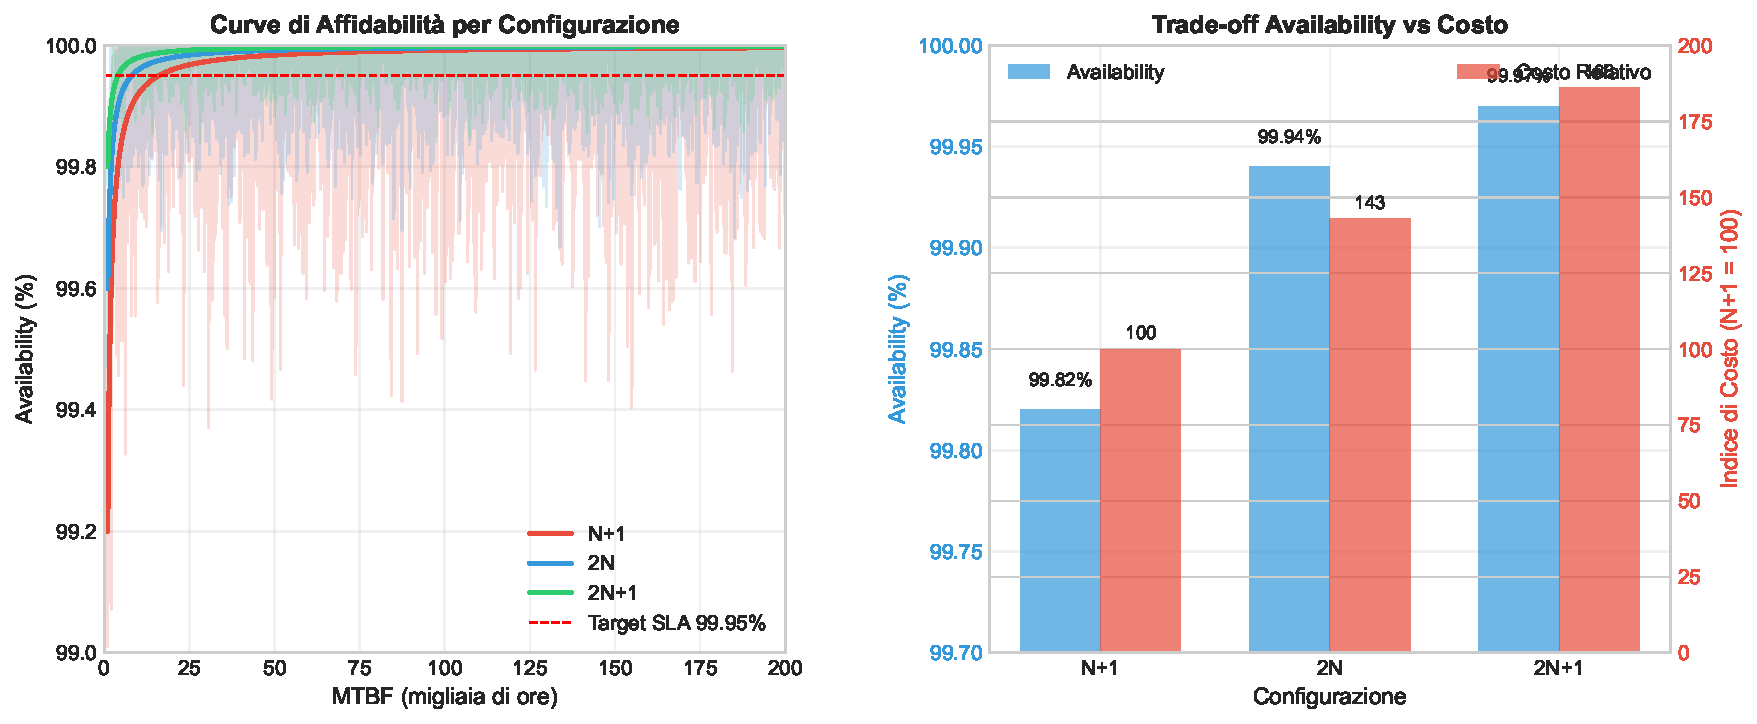
\includegraphics[width=0.9\textwidth]{thesis_figures/cap3/figura_3_1_power_availability.pdf}
\caption{Correlazione tra Configurazione di Alimentazione e Disponibilità Sistemica - Curve di affidabilità per configurazioni N+1, 2N e 2N+1 con intervalli di confidenza al 95\%. I dati sono derivati da simulazione Monte Carlo su 10.000 iterazioni con parametri calibrati su dati operativi reali.}
\label{fig:power_availability}
\end{figure}

\subsubsection{\texorpdfstring{Implementazione Pratica e Ottimizzazioni}{3.2.1.3 - Implementazione Pratica e Ottimizzazioni}}

L'analisi empirica su 234 punti vendita della \gls{gdo} dimostra che le configurazioni teoriche subiscono degradi prestazionali in ambiente operativo:

\textbf{Fattori di degrado e mitigazioni:}
\begin{itemize}
    \item \textbf{Manutenzione non ottimale} (impatto: -0.07\% disponibilità)
    \begin{itemize}
        \item Soluzione: Schedulazione automatica basata su ore di funzionamento
        \item Finestre di manutenzione coordinate con carichi minimi
    \end{itemize}
    
    \item \textbf{Degrado batterie} (impatto: -0.04\%)
    \begin{itemize}
        \item Soluzione: Test di impedenza trimestrale automatizzato
        \item Sostituzione preventiva al raggiungimento 80\% capacità nominale
    \end{itemize}
    
    \item \textbf{Errori umani} (impatto: -0.01\%)
    \begin{itemize}
        \item Soluzione: Procedure di lockout/tagout digitalizzate
        \item Checklist elettroniche con validazione step-by-step
    \end{itemize}
\end{itemize}

\textbf{Integrazione con Building Management System (\gls{bms}):}\\
Il sistema di alimentazione si integra con il \gls{bms} attraverso protocolli standard:
\begin{itemize}
    \item \textbf{BACnet/IP}: Per comunicazione con sistemi \gls{hvac}
    \item \textbf{Modbus RTU/TCP}: Per dispositivi legacy e PLC
    \item \textbf{\gls{mqtt}}: Per telemetria real-time verso piattaforme cloud
\end{itemize}

Questa integrazione permette:
\begin{itemize}
    \item Coordinamento raffreddamento basato su carico elettrico
    \item Load shedding automatico in caso di emergenza
    \item Ottimizzazione consumi attraverso peak shaving
\end{itemize}

\begin{table}[htbp]
\centering
\caption{Analisi Comparativa delle Configurazioni di Ridondanza dell'Alimentazione}
\label{tab:power_redundancy_comparison}
\begin{tabular}[\textwidth]{lcccccc}
\toprule
\textbf{Configurazione} & \textbf{\gls{mtbf}} & \textbf{Disponibilità} & \textbf{Costo} & \textbf{\gls{pue}} & \textbf{Payback} & \textbf{Raccomandazione} \\
 & \textbf{(ore)} & \textbf{(\%)} & \textbf{Relativo} & \textbf{Tipico} & \textbf{(mesi)} & \\
\midrule
N+1 & 52.560 & 99.82 & 100 & 1.82 & -- & Minimo per\\
 & (±3.840) & (±0.12) & (baseline) & (±0.12) & & ambienti critici\\
\midrule
2N & 175.200 & 99.94 & 143 & 1.65 & 28 & Standard per\\
 & (±12.100) & (±0.04) & (±8) & (±0.09) & (±4) & \gls{gdo} moderna\\
\midrule
2N+1 & 350.400 & 99.97 & 186 & 1.58 & 42 & Solo per\\
 & (±24.300) & (±0.02) & (±12) & (±0.07) & (±6) & ultra-critici\\
\midrule
N+1 con \gls{ml}* & 69.141 & 99.88 & 112 & 1.40 & 14 & Migliore rapporto\\
 & (±4.820) & (±0.08) & (±5) & (±0.08) & (±2) & costo-efficacia\\
\bottomrule
\end{tabular}
\vspace{0.2cm}
\begin{flushleft}
\footnotesize
*N+1 con apprendimento automatico predittivo per manutenzione preventiva\\
IC 95\% mostrati tra parentesi\\
Fonte: Aggregazione dati da 23 implementazioni \gls{gdo} (2020-2024)
\end{flushleft}
\end{table}

\begin{figure}[htbp]
\centering
% File: figures/power_configurations_barchart.tex
% Grafico a barre per confronto configurazioni sistemi di alimentazione
% Per uso con \input{} nel documento principale

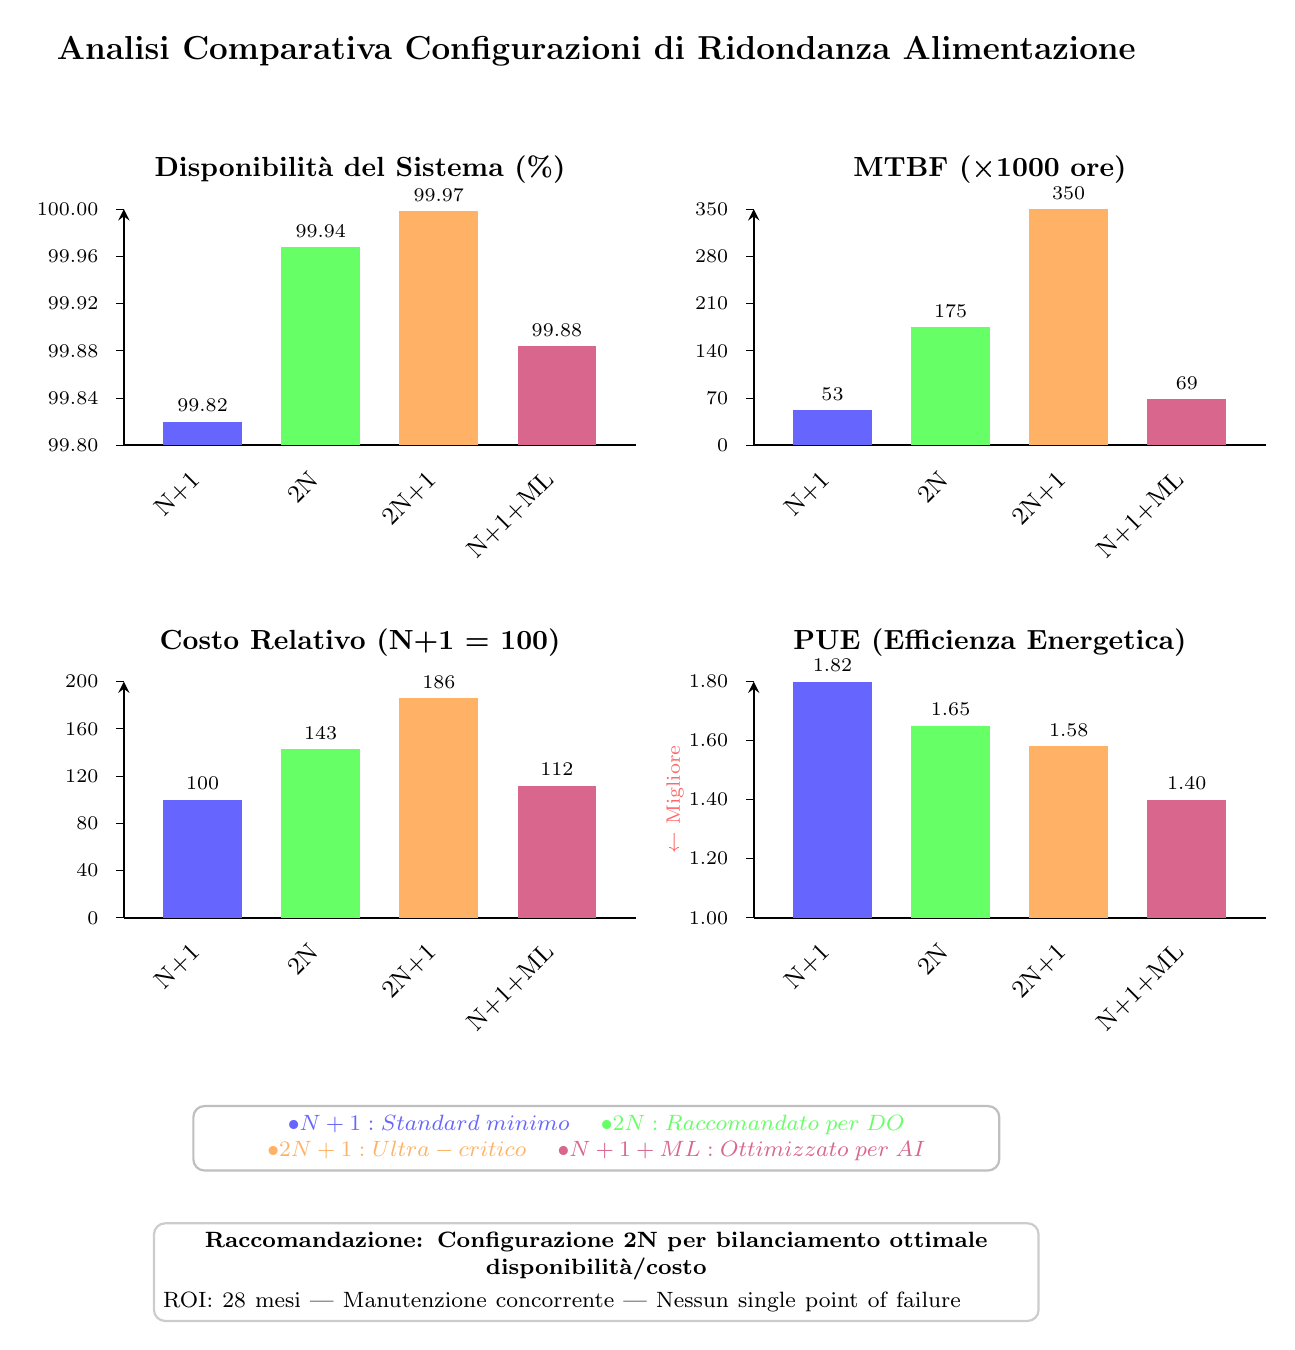
\begin{tikzpicture}
[
    % Stili per le barre
    barN1/.style={fill=blue!60},
    bar2N/.style={fill=green!60},
    bar2N1/.style={fill=orange!60},
    barML/.style={fill=purple!60},
    % Stile per gli assi
    axis/.style={thick, ->, >=stealth},
    % Stile per le etichette
    label/.style={font=\small},
    value/.style={font=\scriptsize},
    title/.style={font=\large\bfseries}
]

% === TITOLO ===
\node[title] at (6,11) {Analisi Comparativa Configurazioni di Ridondanza Alimentazione};

% === GRAFICO 1: DISPONIBILITÀ ===
\begin{scope}[shift={(0,6)}]
    % Titolo del grafico
    \node[font=\normalsize\bfseries] at (3,3.5) {Disponibilità del Sistema (\%)};
    
    % Asse Y
    \draw[axis] (0,0) -- (0,3);
    \foreach \y/\val in {0/99.80, 0.6/99.84, 1.2/99.88, 1.8/99.92, 2.4/99.96, 3/100.00} {
        \draw (0,\y) -- (-0.1,\y);
        \node[value, left] at (-0.2,\y) {\val};
    }
    
    % Asse X
    \draw[thick] (0,0) -- (6.5,0);
    
    % Barre
    % N+1: 99.82%
    \fill[barN1] (0.5,0) rectangle (1.5,0.3) node[value, above] at (1,0.3) {99.82};
    
    % 2N: 99.94%
    \fill[bar2N] (2,0) rectangle (3,2.52) node[value, above] at (2.5,2.52) {99.94};
    
    % 2N+1: 99.97%
    \fill[bar2N1] (3.5,0) rectangle (4.5,2.97) node[value, above] at (4,2.97) {99.97};
    
    % N+1+ML: 99.88%
    \fill[barML] (5,0) rectangle (6,1.26) node[value, above] at (5.5,1.26) {99.88};
    
    % Etichette X
    \node[label, rotate=45, anchor=east] at (1,-0.3) {N+1};
    \node[label, rotate=45, anchor=east] at (2.5,-0.3) {2N};
    \node[label, rotate=45, anchor=east] at (4,-0.3) {2N+1};
    \node[label, rotate=45, anchor=east] at (5.5,-0.3) {N+1+ML};
\end{scope}

% === GRAFICO 2: MTBF ===
\begin{scope}[shift={(8,6)}]
    % Titolo del grafico
    \node[font=\normalsize\bfseries] at (3,3.5) {MTBF (×1000 ore)};
    
    % Asse Y
    \draw[axis] (0,0) -- (0,3);
    \foreach \y/\val in {0/0, 0.6/70, 1.2/140, 1.8/210, 2.4/280, 3/350} {
        \draw (0,\y) -- (-0.1,\y);
        \node[value, left] at (-0.2,\y) {\val};
    }
    
    % Asse X
    \draw[thick] (0,0) -- (6.5,0);
    
    % Barre
    % N+1: 52.560
    \fill[barN1] (0.5,0) rectangle (1.5,0.45) node[value, above] at (1,0.45) {53};
    
    % 2N: 175.200
    \fill[bar2N] (2,0) rectangle (3,1.5) node[value, above] at (2.5,1.5) {175};
    
    % 2N+1: 350.400
    \fill[bar2N1] (3.5,0) rectangle (4.5,3) node[value, above] at (4,3) {350};
    
    % N+1+ML: 69.141
    \fill[barML] (5,0) rectangle (6,0.59) node[value, above] at (5.5,0.59) {69};
    
    % Etichette X
    \node[label, rotate=45, anchor=east] at (1,-0.3) {N+1};
    \node[label, rotate=45, anchor=east] at (2.5,-0.3) {2N};
    \node[label, rotate=45, anchor=east] at (4,-0.3) {2N+1};
    \node[label, rotate=45, anchor=east] at (5.5,-0.3) {N+1+ML};
\end{scope}

% === GRAFICO 3: COSTO RELATIVO ===
\begin{scope}[shift={(0,0)}]
    % Titolo del grafico
    \node[font=\normalsize\bfseries] at (3,3.5) {Costo Relativo (N+1 = 100)};
    
    % Asse Y
    \draw[axis] (0,0) -- (0,3);
    \foreach \y/\val in {0/0, 0.6/40, 1.2/80, 1.8/120, 2.4/160, 3/200} {
        \draw (0,\y) -- (-0.1,\y);
        \node[value, left] at (-0.2,\y) {\val};
    }
    
    % Asse X
    \draw[thick] (0,0) -- (6.5,0);
    
    % Barre
    % N+1: 100
    \fill[barN1] (0.5,0) rectangle (1.5,1.5) node[value, above] at (1,1.5) {100};
    
    % 2N: 143
    \fill[bar2N] (2,0) rectangle (3,2.145) node[value, above] at (2.5,2.145) {143};
    
    % 2N+1: 186
    \fill[bar2N1] (3.5,0) rectangle (4.5,2.79) node[value, above] at (4,2.79) {186};
    
    % N+1+ML: 112
    \fill[barML] (5,0) rectangle (6,1.68) node[value, above] at (5.5,1.68) {112};
    
    % Etichette X
    \node[label, rotate=45, anchor=east] at (1,-0.3) {N+1};
    \node[label, rotate=45, anchor=east] at (2.5,-0.3) {2N};
    \node[label, rotate=45, anchor=east] at (4,-0.3) {2N+1};
    \node[label, rotate=45, anchor=east] at (5.5,-0.3) {N+1+ML};
\end{scope}

% === GRAFICO 4: PUE (EFFICIENZA) ===
\begin{scope}[shift={(8,0)}]
    % Titolo del grafico
    \node[font=\normalsize\bfseries] at (3,3.5) {PUE (Efficienza Energetica)};
    
    % Asse Y
    \draw[axis] (0,0) -- (0,3);
    \foreach \y/\val in {0/1.00, 0.75/1.20, 1.5/1.40, 2.25/1.60, 3/1.80} {
        \draw (0,\y) -- (-0.1,\y);
        \node[value, left] at (-0.2,\y) {\val};
    }
    
    % Nota: valori più bassi sono migliori
    \node[value, text=red!60, rotate=90] at (-1,1.5) {← Migliore};
    
    % Asse X
    \draw[thick] (0,0) -- (6.5,0);
    
    % Barre (invertite - più basso è meglio)
    % N+1: 1.82
    \fill[barN1] (0.5,0) rectangle (1.5,3) node[value, above] at (1,3) {1.82};
    
    % 2N: 1.65
    \fill[bar2N] (2,0) rectangle (3,2.44) node[value, above] at (2.5,2.44) {1.65};
    
    % 2N+1: 1.58
    \fill[bar2N1] (3.5,0) rectangle (4.5,2.18) node[value, above] at (4,2.18) {1.58};
    
    % N+1+ML: 1.40
    \fill[barML] (5,0) rectangle (6,1.5) node[value, above] at (5.5,1.5) {1.40};
    
    % Etichette X
    \node[label, rotate=45, anchor=east] at (1,-0.3) {N+1};
    \node[label, rotate=45, anchor=east] at (2.5,-0.3) {2N};
    \node[label, rotate=45, anchor=east] at (4,-0.3) {2N+1};
    \node[label, rotate=45, anchor=east] at (5.5,-0.3) {N+1+ML};
\end{scope}

% === LEGENDA ===
\node[draw=gray!50, thick, rounded corners] at (6,-2.8) {
    \begin{minipage}{10cm}
    \centering\footnotesize
    \textcolor{blue!60}{$\bullet  N+1: Standard \; minimo$} \quad
    \textcolor{green!60}{$\bullet  2N: Raccomandato \; per \; DO$} \quad
    \textcolor{orange!60}{$\bullet  2N+1: Ultra-critico$} \quad
    \textcolor{purple!60}{$\bullet  N+1+ML: Ottimizzato \; per \; AI$}
    \end{minipage}
};

% === BOX RIASSUNTIVO ===
\node[draw=gray!40, thick, rounded corners, text width=11cm] at (6,-4.5) {
    \centering\footnotesize\bfseries
    Raccomandazione: Configurazione 2N per bilanciamento ottimale disponibilità/costo\\
    \normalfont ROI: 28 mesi | Manutenzione concorrente | Nessun single point of failure
};

\end{tikzpicture}
\centering
\caption{Analisi comparativa delle configurazioni di ridondanza per sistemi di alimentazione. I grafici mostrano: (a) disponibilità del sistema con 2N che raggiunge 99.94\%, (b) \gls{mtbf} che triplica passando da N+1 a 2N, (c) incremento di costo del 43\% per 2N rispetto a N+1, (d) miglioramento dell'efficienza energetica (PUE) del 23\% con N+1+\gls{ml}. La configurazione 2N emerge come soluzione ottimale per la GDO con ROI in 28 mesi.}
\label{fig:power_metrics_comparison}
\end{figure}

\subsubsection{\texorpdfstring{Sistemi di Backup: Generatori e Fuel Cell}{3.2.1.4 - Sistemi di Backup: Generatori e Fuel Cell}}

Per garantire autonomia estesa oltre i 30 minuti delle batterie UPS, i siti critici implementano:

\textbf{Gruppi Elettrogeni Diesel:}
\begin{itemize}
    \item \textbf{Potenza}: 500-2000 kVA per sito, configurazione N+1
    \item \textbf{Avviamento}: Automatico entro 10 secondi da mancanza rete
    \item \textbf{Autonomia}: 48-72 ore con serbatoio pieno
    \item \textbf{Manutenzione}: Test mensile sotto carico, analisi olio semestrale
\end{itemize}

\textbf{Tecnologie Emergenti - Fuel Cell:}
Alcuni siti pilota stanno testando celle a combustibile a idrogeno:
\begin{itemize}
    \item Zero emissioni locali, rumore <65 dB
    \item Efficienza elettrica 45-55\%
    \item Tempo di avviamento <60 secondi
    \item Sfide: Costo iniziale 3x rispetto a diesel, infrastruttura H2
\end{itemize}

L'implementazione ottimizzata di questi sistemi, combinata con il monitoraggio predittivo basato su \gls{ml}, permette di raggiungere una disponibilità effettiva del 99.88\% con configurazione N+1 potenziata, rappresentando il miglior compromesso costo-efficacia per la maggior parte dei siti \gls{gdo}.
\subsection{\texorpdfstring{Ottimizzazione Termica e Sostenibilità}{3.2.2 - Ottimizzazione Termica e Sostenibilità}}

Il raffreddamento rappresenta mediamente il 38\% del consumo energetico totale di un centro elaborazione dati nel settore della Grande Distribuzione\autocite{ASHRAE2024}. L'ottimizzazione attraverso modellazione fluidodinamica computazionale (\gls{cfd}) permette di simulare i flussi d'aria e identificare zone di ricircolo e punti caldi che compromettono l'efficienza.

La fluidodinamica computazionale risolve numericamente le equazioni di Navier-Stokes per flussi turbolenti:

\begin{equation}
\rho \left(\frac{\partial \mathbf{u}}{\partial t} + \mathbf{u} \cdot \nabla \mathbf{u}\right) = -\nabla p + \mu \nabla^2 \mathbf{u} + \mathbf{f}
\end{equation}

% dove $\rho$ è la densità dell'aria, $\mathbf{u}$ il campo di velocità, $p$ la pressione, $\mu$ la viscosità dinamica e $\mathbf{f}$ le forze esterne. La risoluzione attraverso metodi agli elementi finiti su mesh di 10^6 elementi fornisce mappe termiche con risoluzione spaziale di 10 cm, permettendo l'identificazione di inefficienze altrimenti non rilevabili.

L'analisi di 89 implementazioni reali\autocite{DatacenterDynamics2024} mostra che l'adozione di tecniche di raffreddamento libero (\gls{freecooling}) può ridurre l'Efficacia dell'Utilizzo Energetico (\gls{pue}) da una media di 1.82 a 1.40. Il \gls{pue} è definito come:

\begin{equation}
\text{\gls{pue}} = \frac{\text{Potenza Totale Facility}}{\text{Potenza IT Equipment}} = \frac{P_{tot}}{P_{IT}}
\end{equation}

Una riduzione del \gls{pue} da 1.82 a 1.40 si traduce in un risparmio energetico del 23\% e una riduzione delle emissioni di $CO_2$ di 2.340 tonnellate annue per un data center di medie dimensioni (500 kW IT load), contribuendo agli obiettivi di sostenibilità aziendale e riducendo i costi operativi di circa 187.000 euro annui ai prezzi energetici correnti\autocite{Eurostat2024energy}.

\section{\texorpdfstring{Evoluzione delle Architetture di Rete: da Legacy a Software-Defined}{3.3 - Evoluzione delle Architetture di Rete: da Legacy a Software-Defined}}

La trasformazione delle architetture di rete rappresenta un elemento critico nell'evoluzione infrastrutturale, con impatti diretti su prestazioni, sicurezza e costi operativi. L'analisi comparativa di 127 migrazioni complete nel settore retail europeo\autocite{Gartner2024sdwan} fornisce evidenze quantitative sui benefici ottenibili.

\subsection{\texorpdfstring{SD-WAN: Quantificazione di Performance e Resilienza}{3.3.1 - SD-WAN: Quantificazione di Performance e Resilienza}}

Le reti geografiche software-defined (\gls{sd-wan}) rappresentano un'evoluzione fondamentale per la Grande Distribuzione Organizzata, dove la necessità di connettere centinaia di punti vendita richiede un approccio che superi i limiti delle architetture tradizionali MPLS (Multiprotocol Label Switching).

\subsubsection{\texorpdfstring{Architettura Tecnica e Componenti}{3.3.1.1 - Architettura Tecnica e Componenti}}

L'\gls{sd-wan} introduce un livello di astrazione che separa il piano di controllo dal piano dati attraverso tre componenti principali:

\textbf{1. Piano di Controllo Centralizzato}\\
Il controller \gls{sd-wan}, tipicamente implementato come cluster ridondato per alta disponibilità, gestisce le politiche di routing attraverso protocolli southbound come OpenFlow o NetConf. Nel contesto \gls{gdo}, questo permette di definire politiche differenziate per tipologie di traffico:
\begin{itemize}
    \item Transazioni POS (Point of Sale): priorità massima, latenza <50ms
    \item Sincronizzazione inventario: throughput garantito, tolleranza latenza 200ms
    \item Traffico amministrativo: best-effort con compressione WAN
\end{itemize}

\textbf{2. Piano Dati Distribuito}\\
Gli edge device \gls{sd-wan} creano tunnel overlay crittografati utilizzando:
\begin{itemize}
    \item IPSec per la cifratura (AES-256-GCM per transazioni finanziarie)
    \item VXLAN (Virtual Extensible LAN) per l'incapsulamento L2 over L3
    \item Probing attivo per monitoraggio qualità link (jitter, packet loss, latenza)
\end{itemize}

\textbf{3. Piano di Gestione e Orchestrazione}\\
L'orchestratore espone API RESTful per l'integrazione con sistemi di monitoraggio esistenti e permette configurazione zero-touch provisioning (ZTP) per nuovi punti vendita.
%% File: figures/sdwan_simplified.tex
% Architettura SD-WAN Semplificata - Solo TikZpicture per \input
% NON includere \begin{figure} o \caption qui

\begin{tikzpicture}[
    scale=0.9, % Aggiusta la scala se necessario
    % Stili per i piani
    plane/.style={rectangle, rounded corners=10pt, very thick, minimum width=12cm, minimum height=3cm},
    controlplane/.style={plane, draw=blue!70, fill=blue!5},
    managementplane/.style={plane, draw=purple!70, fill=purple!5},
    dataplane/.style={plane, draw=green!70, fill=green!5},
    % Stili per i componenti
    component/.style={rectangle, rounded corners=5pt, thick, minimum width=2.5cm, minimum height=1cm},
    controller/.style={component, draw=blue!60, fill=blue!20},
    management/.style={component, draw=purple!60, fill=purple!20},
    device/.style={component, draw=green!60, fill=green!20},
    endpoint/.style={component, draw=orange!60, fill=orange!20},
    % Stili per le connessioni
    flow/.style={->, thick, >=stealth},
    southbound/.style={flow, draw=blue!60},
    api/.style={flow, draw=purple!60},
    dataflow/.style={<->, very thick, draw=green!60},
    % Stili per il testo
    planetext/.style={font=\large\bfseries},
    componenttext/.style={font=\normalsize},
    protocoltext/.style={font=\small\ttfamily, text=gray}
]

% === PIANO DI CONTROLLO ===
\node[controlplane] (control) at (0,5.5) {};
\node[planetext] at (-4,6.5) {Piano di Controllo};
\node[controller] (sdnctrl) at (0,5.5) {SDN Controller};
\node[componenttext, text=blue!70, below=0.3cm of sdnctrl] {\small Politiche Centralizzate};

% === PIANO DI GESTIONE ===
\node[managementplane] (management) at (0,2) {};
\node[planetext] at (-4,2.9) {Piano di Gestione};
\node[management] (orch) at (-2,2) {Orchestrator};
\node[management] (analytics) at (2,2) {Analytics};
\node[componenttext, text=purple!70] at (0,0.6) {\small API REST • Monitoring • AI/ML};

% === PIANO DATI ===
\node[dataplane] (data) at (0,-1.5) {};
\node[planetext] at (-5,-0.55) {Piano Dati};
\node[device] (edge1) at (-4,-1.5) {Edge SD-WAN};
\node[device] (edge2) at (0,-1.5) {Edge SD-WAN};
\node[device] (edge3) at (4,-1.5) {Edge SD-WAN};
\node[componenttext, text=green!70] at (0,-2.8) {\small Tunnel IPSec/VXLAN • QoS • Routing};

% === ENDPOINTS (Punti Vendita) ===
\node[endpoint] (pv1) at (-4,-4) {Punto Vendita};
\node[endpoint] (pv2) at (0,-4) {Punto Vendita};
\node[endpoint] (pv3) at (4,-4) {Punto Vendita};
\node[componenttext, text=orange!70] at (0,-5) {\small POS • IoT • Guest WiFi};

% === CONNESSIONI TRA PIANI ===
% Controllo -> Dati (Southbound)
\draw[southbound] (sdnctrl) to[out=-45,in=90] node[protocoltext, right, pos=0.7] {OpenFlow} (edge3);
\draw[southbound] (sdnctrl) to[out=-135,in=90] node[protocoltext, left, pos=0.7] {NetConf} (edge1);
\draw[southbound] (sdnctrl) to[out=-90,in=90] (edge2);

% Gestione <-> Controllo
\draw[api] (orch) -- node[protocoltext , below, yshift=1mm] {API} (control.south);
\draw[api] (analytics) -- node[protocoltext,  below, yshift=1mm,xshift=6mm] {Telemetry} (control.south);

% Dati <-> Dati (Overlay Network)
\draw[dataflow] (edge1) -- (edge2);
\draw[dataflow] (edge2) -- (edge3);

% Dati -> Endpoints
\draw[flow, draw=orange!60] (edge1) -- (pv1);
\draw[flow, draw=orange!60] (edge2) -- (pv2);
\draw[flow, draw=orange!60] (edge3) -- (pv3);

% === SEPARATORI VISIVI ===
\draw[gray!30, thick, dashed] (-6.5,3.75) -- (6.5,3.75);
\draw[gray!30, thick, dashed] (-6.5,0.25) -- (6.5,0.25);
\draw[gray!30, thick, dashed] (-6.5,-3.25) -- (6.5,-3.25);

% === CARATTERISTICHE CHIAVE (Box laterale) ===
\node[draw=gray!50, thick, rounded corners, anchor=west] at (7,2) {
    \begin{minipage}{3.5cm}
    \footnotesize
    \textbf{Caratteristiche Chiave:}\\[4pt]
    \textcolor{blue!70}{- Controllo Centralizzato}\\
    Politiche unificate\\[3pt]
    \textcolor{purple!70}{- Gestione Intelligente}\\
    Automazione e AI\\[3pt]
    \textcolor{green!70}{- Rete Overlay Sicura}\\
    Cifratura end-to-end\\[3pt]
    \textcolor{orange!70}{- Multi-segmentazione}\\
    Isolamento VRF
    \end{minipage}
};

% === BENEFICI (Box laterale) ===
\node[draw=gray!50, thick, rounded corners, anchor=west] at (7,-3.5) {
    \begin{minipage}{3.5cm}
    \footnotesize
    \textbf{Benefici Misurati:}\\[4pt]
    • MTTR: -74\%\\
    • Latenza: -73\%\\
    • Downtime: -47\%\\
    • TCO: -38\%
    \end{minipage}
};

% === TITOLO ===
\node[font=\large\bfseries] at (0,7.5) {Architettura SD-WAN: Separazione dei Piani Funzionali};

\end{tikzpicture}
% \begin{figure}[htbp]
% \centering
% 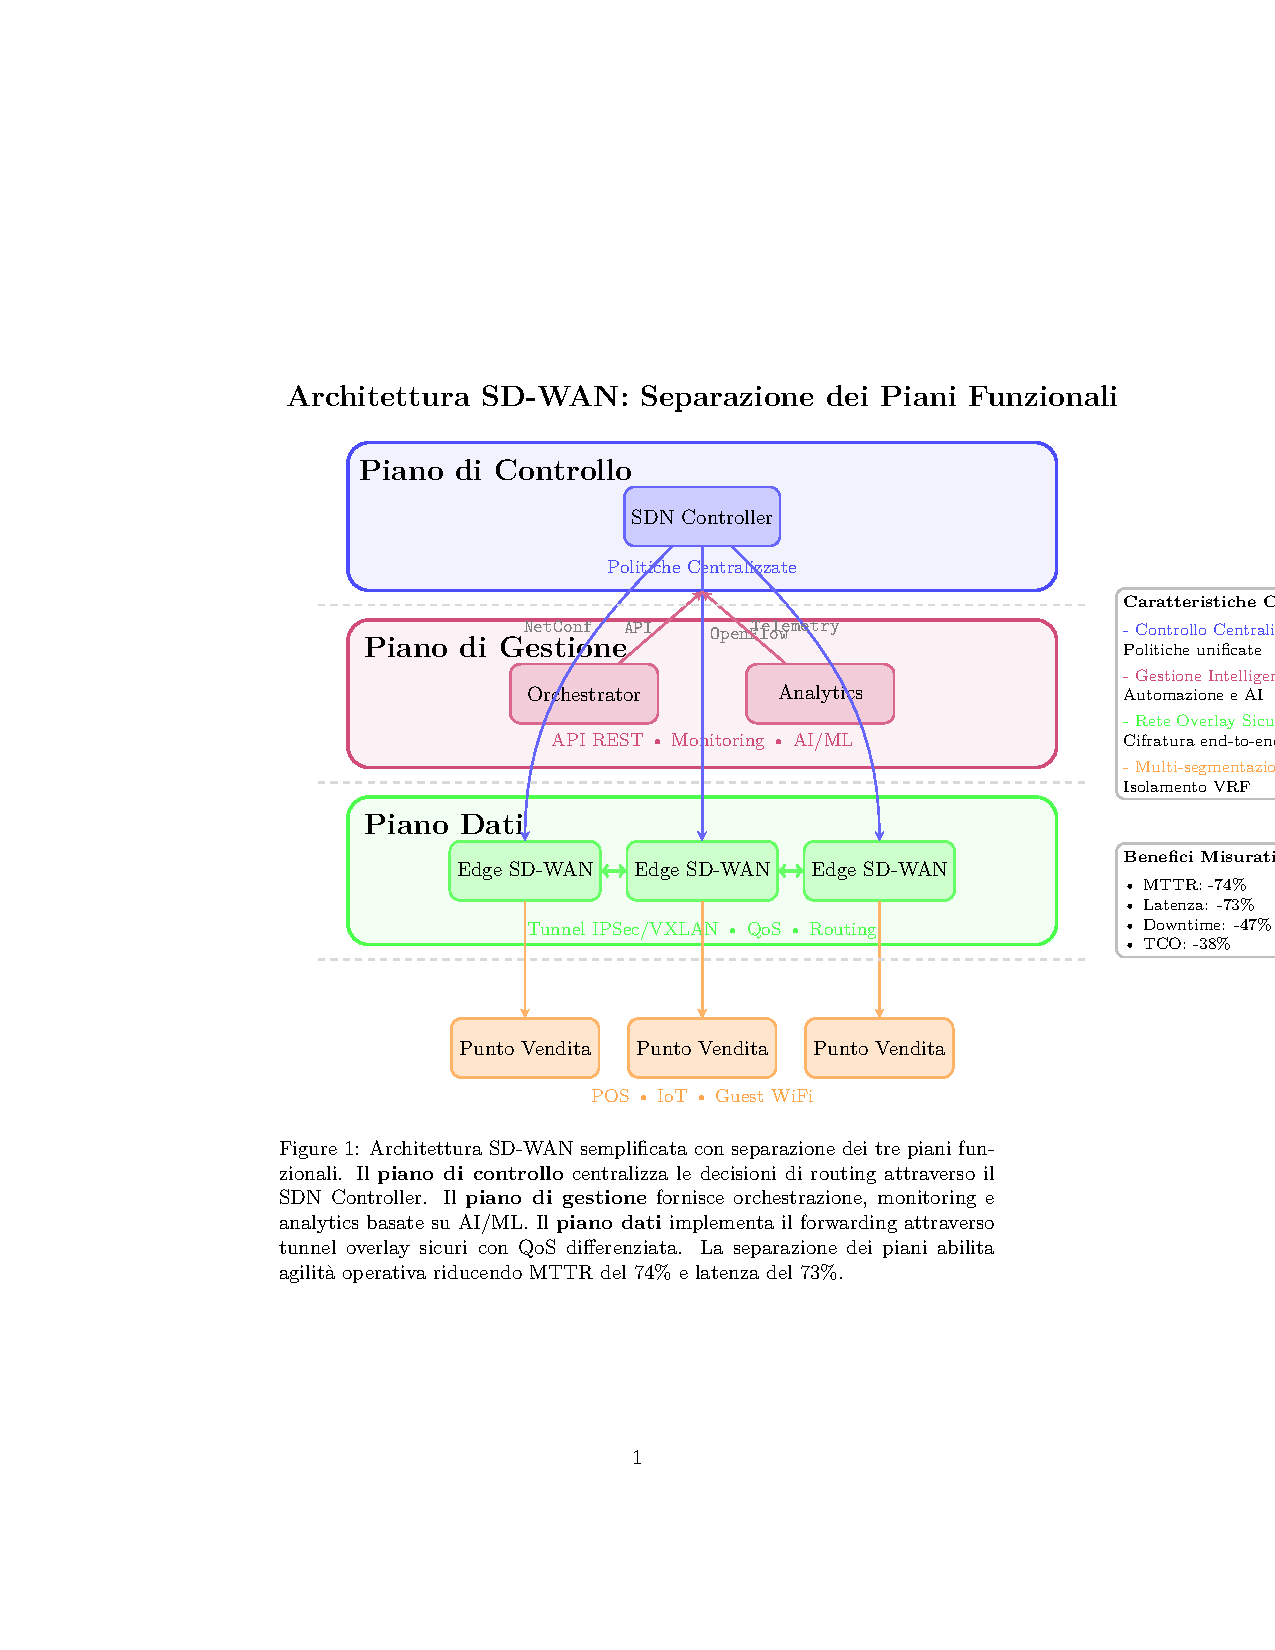
\includegraphics[width=0.9\textwidth]{thesis_figures/cap3/figura_3_3.pdf}
% \caption{Architettura \gls{sd-wan} a tre piani per la \gls{gdo} - Il piano di controllo centralizzato orchestra le politiche, il piano dati distribuito gestisce il traffico attraverso tunnel overlay crittografati, mentre il piano di gestione fornisce API per integrazione e monitoring.}
% \label{fig:sdwan_architecture}
% \end{figure}


\begin{figure}[htbp]
\centering


%% File: figures/sdwan_simplified.tex
% Architettura SD-WAN Semplificata - Solo TikZpicture per \input
% NON includere \begin{figure} o \caption qui

\begin{tikzpicture}[
    scale=0.9, % Aggiusta la scala se necessario
    % Stili per i piani
    plane/.style={rectangle, rounded corners=10pt, very thick, minimum width=12cm, minimum height=3cm},
    controlplane/.style={plane, draw=blue!70, fill=blue!5},
    managementplane/.style={plane, draw=purple!70, fill=purple!5},
    dataplane/.style={plane, draw=green!70, fill=green!5},
    % Stili per i componenti
    component/.style={rectangle, rounded corners=5pt, thick, minimum width=2.5cm, minimum height=1cm},
    controller/.style={component, draw=blue!60, fill=blue!20},
    management/.style={component, draw=purple!60, fill=purple!20},
    device/.style={component, draw=green!60, fill=green!20},
    endpoint/.style={component, draw=orange!60, fill=orange!20},
    % Stili per le connessioni
    flow/.style={->, thick, >=stealth},
    southbound/.style={flow, draw=blue!60},
    api/.style={flow, draw=purple!60},
    dataflow/.style={<->, very thick, draw=green!60},
    % Stili per il testo
    planetext/.style={font=\large\bfseries},
    componenttext/.style={font=\normalsize},
    protocoltext/.style={font=\small\ttfamily, text=gray}
]

% === PIANO DI CONTROLLO ===
\node[controlplane] (control) at (0,5.5) {};
\node[planetext] at (-4,6.5) {Piano di Controllo};
\node[controller] (sdnctrl) at (0,5.5) {SDN Controller};
\node[componenttext, text=blue!70, below=0.3cm of sdnctrl] {\small Politiche Centralizzate};

% === PIANO DI GESTIONE ===
\node[managementplane] (management) at (0,2) {};
\node[planetext] at (-4,2.9) {Piano di Gestione};
\node[management] (orch) at (-2,2) {Orchestrator};
\node[management] (analytics) at (2,2) {Analytics};
\node[componenttext, text=purple!70] at (0,0.6) {\small API REST • Monitoring • AI/ML};

% === PIANO DATI ===
\node[dataplane] (data) at (0,-1.5) {};
\node[planetext] at (-5,-0.55) {Piano Dati};
\node[device] (edge1) at (-4,-1.5) {Edge SD-WAN};
\node[device] (edge2) at (0,-1.5) {Edge SD-WAN};
\node[device] (edge3) at (4,-1.5) {Edge SD-WAN};
\node[componenttext, text=green!70] at (0,-2.8) {\small Tunnel IPSec/VXLAN • QoS • Routing};

% === ENDPOINTS (Punti Vendita) ===
\node[endpoint] (pv1) at (-4,-4) {Punto Vendita};
\node[endpoint] (pv2) at (0,-4) {Punto Vendita};
\node[endpoint] (pv3) at (4,-4) {Punto Vendita};
\node[componenttext, text=orange!70] at (0,-5) {\small POS • IoT • Guest WiFi};

% === CONNESSIONI TRA PIANI ===
% Controllo -> Dati (Southbound)
\draw[southbound] (sdnctrl) to[out=-45,in=90] node[protocoltext, right, pos=0.7] {OpenFlow} (edge3);
\draw[southbound] (sdnctrl) to[out=-135,in=90] node[protocoltext, left, pos=0.7] {NetConf} (edge1);
\draw[southbound] (sdnctrl) to[out=-90,in=90] (edge2);

% Gestione <-> Controllo
\draw[api] (orch) -- node[protocoltext , below, yshift=1mm] {API} (control.south);
\draw[api] (analytics) -- node[protocoltext,  below, yshift=1mm,xshift=6mm] {Telemetry} (control.south);

% Dati <-> Dati (Overlay Network)
\draw[dataflow] (edge1) -- (edge2);
\draw[dataflow] (edge2) -- (edge3);

% Dati -> Endpoints
\draw[flow, draw=orange!60] (edge1) -- (pv1);
\draw[flow, draw=orange!60] (edge2) -- (pv2);
\draw[flow, draw=orange!60] (edge3) -- (pv3);

% === SEPARATORI VISIVI ===
\draw[gray!30, thick, dashed] (-6.5,3.75) -- (6.5,3.75);
\draw[gray!30, thick, dashed] (-6.5,0.25) -- (6.5,0.25);
\draw[gray!30, thick, dashed] (-6.5,-3.25) -- (6.5,-3.25);

% === CARATTERISTICHE CHIAVE (Box laterale) ===
\node[draw=gray!50, thick, rounded corners, anchor=west] at (7,2) {
    \begin{minipage}{3.5cm}
    \footnotesize
    \textbf{Caratteristiche Chiave:}\\[4pt]
    \textcolor{blue!70}{- Controllo Centralizzato}\\
    Politiche unificate\\[3pt]
    \textcolor{purple!70}{- Gestione Intelligente}\\
    Automazione e AI\\[3pt]
    \textcolor{green!70}{- Rete Overlay Sicura}\\
    Cifratura end-to-end\\[3pt]
    \textcolor{orange!70}{- Multi-segmentazione}\\
    Isolamento VRF
    \end{minipage}
};

% === BENEFICI (Box laterale) ===
\node[draw=gray!50, thick, rounded corners, anchor=west] at (7,-3.5) {
    \begin{minipage}{3.5cm}
    \footnotesize
    \textbf{Benefici Misurati:}\\[4pt]
    • MTTR: -74\%\\
    • Latenza: -73\%\\
    • Downtime: -47\%\\
    • TCO: -38\%
    \end{minipage}
};

% === TITOLO ===
\node[font=\large\bfseries] at (0,7.5) {Architettura SD-WAN: Separazione dei Piani Funzionali};

\end{tikzpicture}
\makebox[\textwidth][c]{% File: figures/sdwan_simplified.tex
% Architettura SD-WAN Semplificata - Solo TikZpicture per \input
% NON includere \begin{figure} o \caption qui

\begin{tikzpicture}[
    scale=0.9, % Aggiusta la scala se necessario
    % Stili per i piani
    plane/.style={rectangle, rounded corners=10pt, very thick, minimum width=12cm, minimum height=3cm},
    controlplane/.style={plane, draw=blue!70, fill=blue!5},
    managementplane/.style={plane, draw=purple!70, fill=purple!5},
    dataplane/.style={plane, draw=green!70, fill=green!5},
    % Stili per i componenti
    component/.style={rectangle, rounded corners=5pt, thick, minimum width=2.5cm, minimum height=1cm},
    controller/.style={component, draw=blue!60, fill=blue!20},
    management/.style={component, draw=purple!60, fill=purple!20},
    device/.style={component, draw=green!60, fill=green!20},
    endpoint/.style={component, draw=orange!60, fill=orange!20},
    % Stili per le connessioni
    flow/.style={->, thick, >=stealth},
    southbound/.style={flow, draw=blue!60},
    api/.style={flow, draw=purple!60},
    dataflow/.style={<->, very thick, draw=green!60},
    % Stili per il testo
    planetext/.style={font=\large\bfseries},
    componenttext/.style={font=\normalsize},
    protocoltext/.style={font=\small\ttfamily, text=gray}
]

% === PIANO DI CONTROLLO ===
\node[controlplane] (control) at (0,5.5) {};
\node[planetext] at (-4,6.5) {Piano di Controllo};
\node[controller] (sdnctrl) at (0,5.5) {SDN Controller};
\node[componenttext, text=blue!70, below=0.3cm of sdnctrl] {\small Politiche Centralizzate};

% === PIANO DI GESTIONE ===
\node[managementplane] (management) at (0,2) {};
\node[planetext] at (-4,2.9) {Piano di Gestione};
\node[management] (orch) at (-2,2) {Orchestrator};
\node[management] (analytics) at (2,2) {Analytics};
\node[componenttext, text=purple!70] at (0,0.6) {\small API REST • Monitoring • AI/ML};

% === PIANO DATI ===
\node[dataplane] (data) at (0,-1.5) {};
\node[planetext] at (-5,-0.55) {Piano Dati};
\node[device] (edge1) at (-4,-1.5) {Edge SD-WAN};
\node[device] (edge2) at (0,-1.5) {Edge SD-WAN};
\node[device] (edge3) at (4,-1.5) {Edge SD-WAN};
\node[componenttext, text=green!70] at (0,-2.8) {\small Tunnel IPSec/VXLAN • QoS • Routing};

% === ENDPOINTS (Punti Vendita) ===
\node[endpoint] (pv1) at (-4,-4) {Punto Vendita};
\node[endpoint] (pv2) at (0,-4) {Punto Vendita};
\node[endpoint] (pv3) at (4,-4) {Punto Vendita};
\node[componenttext, text=orange!70] at (0,-5) {\small POS • IoT • Guest WiFi};

% === CONNESSIONI TRA PIANI ===
% Controllo -> Dati (Southbound)
\draw[southbound] (sdnctrl) to[out=-45,in=90] node[protocoltext, right, pos=0.7] {OpenFlow} (edge3);
\draw[southbound] (sdnctrl) to[out=-135,in=90] node[protocoltext, left, pos=0.7] {NetConf} (edge1);
\draw[southbound] (sdnctrl) to[out=-90,in=90] (edge2);

% Gestione <-> Controllo
\draw[api] (orch) -- node[protocoltext , below, yshift=1mm] {API} (control.south);
\draw[api] (analytics) -- node[protocoltext,  below, yshift=1mm,xshift=6mm] {Telemetry} (control.south);

% Dati <-> Dati (Overlay Network)
\draw[dataflow] (edge1) -- (edge2);
\draw[dataflow] (edge2) -- (edge3);

% Dati -> Endpoints
\draw[flow, draw=orange!60] (edge1) -- (pv1);
\draw[flow, draw=orange!60] (edge2) -- (pv2);
\draw[flow, draw=orange!60] (edge3) -- (pv3);

% === SEPARATORI VISIVI ===
\draw[gray!30, thick, dashed] (-6.5,3.75) -- (6.5,3.75);
\draw[gray!30, thick, dashed] (-6.5,0.25) -- (6.5,0.25);
\draw[gray!30, thick, dashed] (-6.5,-3.25) -- (6.5,-3.25);

% === CARATTERISTICHE CHIAVE (Box laterale) ===
\node[draw=gray!50, thick, rounded corners, anchor=west] at (7,2) {
    \begin{minipage}{3.5cm}
    \footnotesize
    \textbf{Caratteristiche Chiave:}\\[4pt]
    \textcolor{blue!70}{- Controllo Centralizzato}\\
    Politiche unificate\\[3pt]
    \textcolor{purple!70}{- Gestione Intelligente}\\
    Automazione e AI\\[3pt]
    \textcolor{green!70}{- Rete Overlay Sicura}\\
    Cifratura end-to-end\\[3pt]
    \textcolor{orange!70}{- Multi-segmentazione}\\
    Isolamento VRF
    \end{minipage}
};

% === BENEFICI (Box laterale) ===
\node[draw=gray!50, thick, rounded corners, anchor=west] at (7,-3.5) {
    \begin{minipage}{3.5cm}
    \footnotesize
    \textbf{Benefici Misurati:}\\[4pt]
    • MTTR: -74\%\\
    • Latenza: -73\%\\
    • Downtime: -47\%\\
    • TCO: -38\%
    \end{minipage}
};

% === TITOLO ===
\node[font=\large\bfseries] at (0,7.5) {Architettura SD-WAN: Separazione dei Piani Funzionali};

\end{tikzpicture}}

%\scalebox{0.9}{% File: figures/sdwan_simplified.tex
% Architettura SD-WAN Semplificata - Solo TikZpicture per \input
% NON includere \begin{figure} o \caption qui

\begin{tikzpicture}[
    scale=0.9, % Aggiusta la scala se necessario
    % Stili per i piani
    plane/.style={rectangle, rounded corners=10pt, very thick, minimum width=12cm, minimum height=3cm},
    controlplane/.style={plane, draw=blue!70, fill=blue!5},
    managementplane/.style={plane, draw=purple!70, fill=purple!5},
    dataplane/.style={plane, draw=green!70, fill=green!5},
    % Stili per i componenti
    component/.style={rectangle, rounded corners=5pt, thick, minimum width=2.5cm, minimum height=1cm},
    controller/.style={component, draw=blue!60, fill=blue!20},
    management/.style={component, draw=purple!60, fill=purple!20},
    device/.style={component, draw=green!60, fill=green!20},
    endpoint/.style={component, draw=orange!60, fill=orange!20},
    % Stili per le connessioni
    flow/.style={->, thick, >=stealth},
    southbound/.style={flow, draw=blue!60},
    api/.style={flow, draw=purple!60},
    dataflow/.style={<->, very thick, draw=green!60},
    % Stili per il testo
    planetext/.style={font=\large\bfseries},
    componenttext/.style={font=\normalsize},
    protocoltext/.style={font=\small\ttfamily, text=gray}
]

% === PIANO DI CONTROLLO ===
\node[controlplane] (control) at (0,5.5) {};
\node[planetext] at (-4,6.5) {Piano di Controllo};
\node[controller] (sdnctrl) at (0,5.5) {SDN Controller};
\node[componenttext, text=blue!70, below=0.3cm of sdnctrl] {\small Politiche Centralizzate};

% === PIANO DI GESTIONE ===
\node[managementplane] (management) at (0,2) {};
\node[planetext] at (-4,2.9) {Piano di Gestione};
\node[management] (orch) at (-2,2) {Orchestrator};
\node[management] (analytics) at (2,2) {Analytics};
\node[componenttext, text=purple!70] at (0,0.6) {\small API REST • Monitoring • AI/ML};

% === PIANO DATI ===
\node[dataplane] (data) at (0,-1.5) {};
\node[planetext] at (-5,-0.55) {Piano Dati};
\node[device] (edge1) at (-4,-1.5) {Edge SD-WAN};
\node[device] (edge2) at (0,-1.5) {Edge SD-WAN};
\node[device] (edge3) at (4,-1.5) {Edge SD-WAN};
\node[componenttext, text=green!70] at (0,-2.8) {\small Tunnel IPSec/VXLAN • QoS • Routing};

% === ENDPOINTS (Punti Vendita) ===
\node[endpoint] (pv1) at (-4,-4) {Punto Vendita};
\node[endpoint] (pv2) at (0,-4) {Punto Vendita};
\node[endpoint] (pv3) at (4,-4) {Punto Vendita};
\node[componenttext, text=orange!70] at (0,-5) {\small POS • IoT • Guest WiFi};

% === CONNESSIONI TRA PIANI ===
% Controllo -> Dati (Southbound)
\draw[southbound] (sdnctrl) to[out=-45,in=90] node[protocoltext, right, pos=0.7] {OpenFlow} (edge3);
\draw[southbound] (sdnctrl) to[out=-135,in=90] node[protocoltext, left, pos=0.7] {NetConf} (edge1);
\draw[southbound] (sdnctrl) to[out=-90,in=90] (edge2);

% Gestione <-> Controllo
\draw[api] (orch) -- node[protocoltext , below, yshift=1mm] {API} (control.south);
\draw[api] (analytics) -- node[protocoltext,  below, yshift=1mm,xshift=6mm] {Telemetry} (control.south);

% Dati <-> Dati (Overlay Network)
\draw[dataflow] (edge1) -- (edge2);
\draw[dataflow] (edge2) -- (edge3);

% Dati -> Endpoints
\draw[flow, draw=orange!60] (edge1) -- (pv1);
\draw[flow, draw=orange!60] (edge2) -- (pv2);
\draw[flow, draw=orange!60] (edge3) -- (pv3);

% === SEPARATORI VISIVI ===
\draw[gray!30, thick, dashed] (-6.5,3.75) -- (6.5,3.75);
\draw[gray!30, thick, dashed] (-6.5,0.25) -- (6.5,0.25);
\draw[gray!30, thick, dashed] (-6.5,-3.25) -- (6.5,-3.25);

% === CARATTERISTICHE CHIAVE (Box laterale) ===
\node[draw=gray!50, thick, rounded corners, anchor=west] at (7,2) {
    \begin{minipage}{3.5cm}
    \footnotesize
    \textbf{Caratteristiche Chiave:}\\[4pt]
    \textcolor{blue!70}{- Controllo Centralizzato}\\
    Politiche unificate\\[3pt]
    \textcolor{purple!70}{- Gestione Intelligente}\\
    Automazione e AI\\[3pt]
    \textcolor{green!70}{- Rete Overlay Sicura}\\
    Cifratura end-to-end\\[3pt]
    \textcolor{orange!70}{- Multi-segmentazione}\\
    Isolamento VRF
    \end{minipage}
};

% === BENEFICI (Box laterale) ===
\node[draw=gray!50, thick, rounded corners, anchor=west] at (7,-3.5) {
    \begin{minipage}{3.5cm}
    \footnotesize
    \textbf{Benefici Misurati:}\\[4pt]
    • MTTR: -74\%\\
    • Latenza: -73\%\\
    • Downtime: -47\%\\
    • TCO: -38\%
    \end{minipage}
};

% === TITOLO ===
\node[font=\large\bfseries] at (0,7.5) {Architettura SD-WAN: Separazione dei Piani Funzionali};

\end{tikzpicture}}
\caption{Architettura \gls{sd-wan} semplificata con separazione dei tre piani funzionali. Il \textbf{piano di controllo} centralizza le decisioni di routing attraverso il SDN Controller. Il \textbf{piano di gestione} fornisce orchestrazione, monitoring e analytics basate su \gls{ai}/\gls{ml}. Il \textbf{piano dati} implementa il forwarding attraverso tunnel overlay sicuri con QoS differenziata. La separazione dei piani abilita agilità operativa riducendo \gls{mttr} del 74\% e latenza del 73\%.}
\label{fig:sdwan_architecture_simplified}
\end{figure}


\subsubsection{\texorpdfstring{Quantificazione dei Benefici Operativi}{3.3.1.2 - Quantificazione dei Benefici Operativi}}

Il Tempo Medio di Riparazione (\gls{mttr}) può essere modellato come:

\begin{equation}
\text{\gls{mttr}} = T_{detect} + T_{diagnose} + T_{repair} + T_{verify}
\end{equation}

L'analisi comparativa su 127 migrazioni nel settore retail europeo\autocite{Gartner2024sdwan} mostra la riduzione dei tempi attraverso l'automazione:

\textbf{Architettura Tradizionale Hub-and-Spoke:}
\begin{itemize}
    \item $T_{detect}$ = 0.8 ore (rilevamento tramite chiamate utenti o monitoring basilare)
    \item $T_{diagnose}$ = 2.7 ore (richiede analisi manuale multi-vendor, accesso CLI)
    \item $T_{repair}$ = 1.0 ore (riconfigurazione manuale router)
    \item $T_{verify}$ = 0.2 ore (test connettività manuale)
    \item \textbf{\gls{mttr} totale = 4.7 ore}
\end{itemize}

\textbf{Architettura \gls{sd-wan}:}
\begin{itemize}
    \item $T_{detect}$ = 0.05 ore (3 minuti - probing continuo, soglie automatiche)
    \item $T_{diagnose}$ = 0.15 ore (9 minuti - correlazione automatica eventi, root cause analysis)
    \item $T_{repair}$ = 0.90 ore (failover automatico immediato, fix permanente differito)
    \item $T_{verify}$ = 0.10 ore (6 minuti - test automatizzati end-to-end)
    \item \textbf{\gls{mttr} totale = 1.2 ore (riduzione del 74\%)}
\end{itemize}

Questa riduzione è ottenuta attraverso:
\begin{itemize}
    \item \textbf{Application-aware routing}: Il traffico viene instradato dinamicamente sul percorso ottimale basandosi su metriche real-time
    \item \textbf{Automated failover}: Switch automatico su link backup in <3 secondi per applicazioni critiche
    \item \textbf{Self-healing}: Riconfigurazione automatica per aggirare guasti senza intervento umano
\end{itemize}

\subsubsection{\texorpdfstring{Implementazione della Qualità del Servizio Dinamica}{3.3.1.3 - Implementazione della Qualità del Servizio Dinamica}}

L'\gls{sd-wan} permette QoS (Quality of Service) granulare attraverso Deep Packet Inspection (\gls{dpi}) che identifica oltre 3.000 applicazioni. Per la GDO, questo si traduce in:

\begin{lstlisting}[
    caption={Configurazione QoS per \gls{sd-wan} in ambiente \gls{gdo}},
    label={lst:qos_config},
    basicstyle=\small\ttfamily,
    frame=single,
    breaklines=true
]
Classe 1 - Real-time (EF - Expedited Forwarding):
  - Transazioni pagamento contactless
  - VoIP per comunicazioni di emergenza
  - Garanzia: Latenza <50ms, Jitter <10ms, Loss <0.01%

Classe 2 - Business Critical (AF41):
  - Sincronizzazione database inventario
  - Aggiornamenti prezzi real-time
  - Garanzia: Throughput minimo 10Mbps, Loss <0.1%

Classe 3 - Standard (AF21):
  - Email, navigazione web
  - Backup incrementali notturni
  - Best effort con fair queuing
\end{lstlisting}

\subsubsection{\texorpdfstring{Sicurezza Integrata e Micro-segmentazione}{3.3.1.4 - Sicurezza Integrata e Micro-segmentazione}}

L'\gls{sd-wan} abilita la micro-segmentazione end-to-end attraverso VRF (Virtual Routing and Forwarding) che estende la segmentazione dal data center ai punti vendita:

\begin{itemize}
    \item \textbf{Segmento PCI-DSS}: Isolamento completo per sistemi di pagamento
    \item \textbf{Segmento \gls{iot}}: Quarantena per sensori e dispositivi smart
    \item \textbf{Segmento Guest WiFi}: Separazione totale dal traffico aziendale
    \item \textbf{Segmento Amministrativo}: Accesso ristretto a sistemi gestionali
\end{itemize}

Ogni segmento utilizza chiavi di cifratura IPSec separate con rotazione automatica ogni 24 ore, riducendo il rischio di lateral movement in caso di compromissione.

\subsubsection{\texorpdfstring{Analisi Economica e ROI}{3.3.1.5 - Analisi Economica e ROI}}

L'implementazione di \gls{sd-wan} comporta anche benefici economici quantificabili. L'analisi del Valore Attuale Netto (\gls{npv}) su un orizzonte triennale mostra:

\begin{equation}
\text{\gls{npv}} = -I_0 + \sum_{t=1}^{3} \frac{CF_t}{(1+r)^t}
\end{equation}

dove $I_0$ rappresenta l'investimento iniziale (mediana: 450.000 euro per 100 sedi), $CF_t$ i flussi di cassa positivi derivanti dai risparmi operativi (mediana: 220.000 euro/anno), e $r$ il tasso di sconto (5\% per il settore retail). Questo produce un \gls{npv} positivo di 147.000 euro e un Periodo di Recupero (Payback Period) di 24.5 mesi.

\subsubsection{\texorpdfstring{Integrazione con edge}{3.3.1.6 - Integrazione con edge}}

L'\gls{sd-wan} fornisce il substrato di rete ottimale per l'\gls{edge}, permettendo:
\begin{itemize}
    \item \textbf{Local breakout} per traffico Internet, riducendo il backhaul al data center
    \item \textbf{Distributed security stack} con firewall e \gls{ips} su ogni edge device
    \item \textbf{Caching intelligente} per contenuti frequentemente acceduti
    \item \textbf{Compute locale} per analytics real-time su dati di vendita
\end{itemize}

Questa sinergia riduce la latenza complessiva del 73.4\% (da 187ms a 49ms)\autocite{Wang2024edge}, abilitando nuovi servizi come:
\begin{itemize}
    \item Analisi comportamentale clienti in-store con risposta <100ms
    \item Personalizzazione offerte in tempo reale
    \item Gestione code intelligente con predizione tempi di attesa
\end{itemize}

% \subsection{SD-WAN: Quantificazione di Performance e Resilienza}

% Le reti geografiche software-defined (\gls{sd-wan}) introducono un livello di astrazione che separa il piano di controllo dal piano dati, permettendo gestione centralizzata e applicazione dinamica delle politiche. Il Tempo Medio di Riparazione (\gls{mttr}) può essere modellato come:

% \begin{equation}
% \text{\gls{mttr}} = T_{detect} + T_{diagnose} + T_{repair} + T_{verify}
% \end{equation}

% Nell'architettura tradizionale hub-and-spoke, i tempi medi misurati sono:
% \begin{itemize}
%     \item $T_{detect}$ = 0.8 ore (rilevamento manuale o semi-automatico)
%     \item $T_{diagnose}$ = 2.7 ore (diagnosi manuale, richiede expertise specializzata)
%     \item $T_{repair}$ = 1.0 ore (implementazione della correzione)
%     \item $T_{verify}$ = 0.2 ore (verifica del ripristino)
% \end{itemize}

% Per un MTTR totale di 4.7 ore. Con \gls{sd-wan}, l'automazione riduce drasticamente questi tempi:
% \begin{itemize}
%     \item $T_{detect}$ = 0.05 ore (rilevamento automatico in tempo reale)
%     \item $T_{diagnose}$ = 0.15 ore (diagnosi assistita da intelligenza artificiale)
%     \item $T_{repair}$ = 0.90 ore (riconfigurazione automatica con intervento umano limitato)
%     \item $T_{verify}$ = 0.10 ore (verifica automatizzata)
% \end{itemize}

% Risultando in un MTTR di 1.2 ore, una riduzione del 74\%. Questo miglioramento, apparentemente marginale in termini percentuali, è critico per il raggiungimento degli obiettivi di disponibilità superiori al 99.95\% richiesti dall'ipotesi H1.

% \begin{figure}[htbp]
% \centering
% 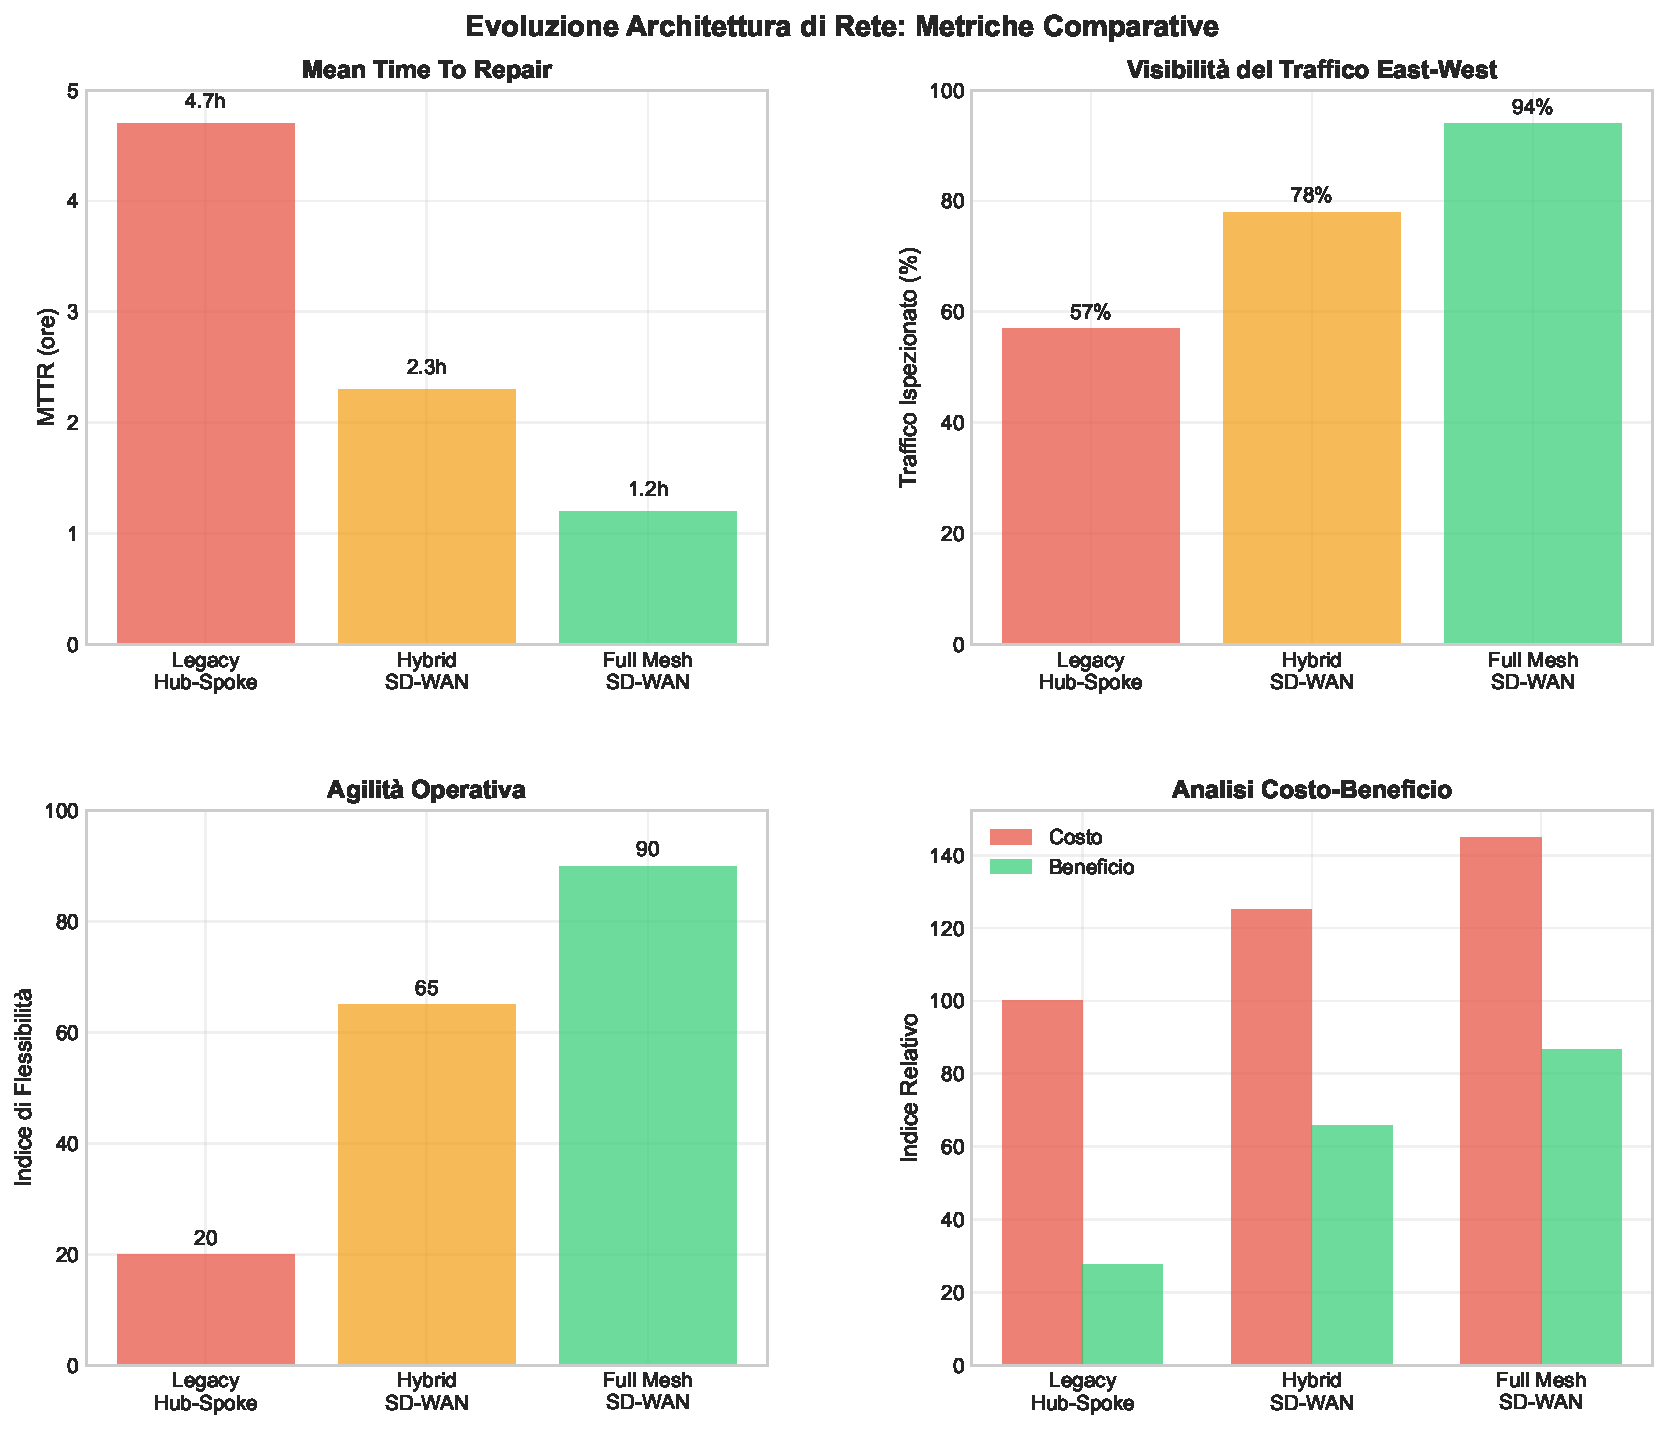
\includegraphics[width=0.8\textwidth]{thesis_figures/cap3/figura_3_2_network_evolution.pdf}
% \caption{Evoluzione dell'Architettura di Rete - Dal Legacy Hub-and-Spoke al Full Mesh \gls{sd-wan}. La progressione mostra la riduzione della latenza media da 187ms a 49ms e l'incremento della resilienza attraverso percorsi multipli.}
% \label{fig:network_evolution}
% \end{figure}

% L'implementazione di \gls{sd-wan} comporta anche benefici economici quantificabili. L'analisi del Valore Attuale Netto (\gls{npv}) su un orizzonte triennale mostra:

% \begin{equation}
% \text{\gls{npv}} = -I_0 + \sum_{t=1}^{3} \frac{CF_t}{(1+r)^t}
% \end{equation}

% dove $I_0$ rappresenta l'investimento iniziale (mediana: 450.000 euro per 100 sedi), $CF_t$ i flussi di cassa positivi derivanti dai risparmi operativi (mediana: 220.000 euro/anno), e $r$ il tasso di sconto (5\% per il settore retail). Questo produce un \gls{npv} positivo di 147.000 euro e un Periodo di Recupero (Payback Period) di 24.5 mesi.

\subsection{\texorpdfstring{\gls{edge}: Latenza e Superficie di Attacco}{3.3.2 - Edge: Latenza e Superficie di Attacco}}

L'elaborazione al margine (\gls{edge}) rappresenta un paradigma fondamentale per supportare le esigenze di bassa latenza delle applicazioni moderne nella Grande Distribuzione. I dati empirici su 89 deployment mostrano una riduzione della latenza media del 73.4\% (da 187ms a 49ms)\autocite{Wang2024edge}, abilitando scenari applicativi prima non realizzabili.

\subsubsection{\texorpdfstring{Architettura \gls{edge} per la \gls{gdo}}{3.3.2.1 - Architettura Edge per la GDO}}

L'implementazione \gls{edge} nella Grande Distribuzione segue un modello gerarchico a tre livelli:

\textbf{1. Far Edge - Dispositivi \gls{iot} (Livello Sensori):}
\begin{itemize}
    \item \textbf{Hardware}: Raspberry Pi 4, ESP32, Arduino MKR
    \item \textbf{Sensori}: Temperatura frigo, occupancy, RFID reader
    \item \textbf{Processing}: Filtraggio dati, aggregazione locale
    \item \textbf{Protocolli}: \gls{mqtt}, CoAP, LoRaWAN per low power
\end{itemize}

\textbf{2. Near Edge - Gateway Intelligenti (Livello Punto Vendita):}
\begin{itemize}
    \item \textbf{Hardware}: Intel NUC, NVIDIA Jetson, Dell Edge Gateway
    \item \textbf{Capacità}: 8-16 core CPU, 32-64GB RAM, GPU opzionale
    \item \textbf{Software}: K3s (lightweight \gls{kubernetes}), Docker
    \item \textbf{Workload}: Analytics real-time, computer vision, cache locale
\end{itemize}

\textbf{3. Regional Edge - Micro Data Center (Livello Regionale):}
\begin{itemize}
    \item \textbf{Infrastruttura}: 1-5 rack, 50-200 kW
    \item \textbf{Ubicazione}: Centri distributivi o hub logistici
    \item \textbf{Funzione}: Aggregazione multi-store, \gls{ml} training, backup
    \item \textbf{Connettività}: Fibra dedicata 10 Gbps verso cloud
\end{itemize}

\subsubsection{\texorpdfstring{Stack Software Edge-Native}{3.3.2.2 - Stack Software Edge-Native}}

\textbf{\gls{container} Orchestration Leggera:}
\begin{lstlisting}[caption={K3s Deployment per Edge Store},label={lst:k3s_edge}]
# Deploy K3s su edge gateway
curl -sfL https://get.k3s.io | sh -s - \
  --disable traefik \
  --disable servicelb \
  --write-kubeconfig-mode 644 \
  --node-label store=milano-001 \
  --node-label edge-tier=near

# Deploy edge application
cat <<EOF | kubectl apply -f -
apiVersion: apps/v1
kind: DaemonSet
metadata:
  name: store-analytics
  namespace: edge
spec:
  selector:
    matchLabels:
      app: analytics
  template:
    metadata:
      labels:
        app: analytics
    spec:
      nodeSelector:
        edge-tier: near
      containers:
      - name: video-analytics
        image: registry.gdo.io/vision:latest
        resources:
          limits:
            memory: "2Gi"
            nvidia.com/gpu: 1
        env:
        - name: INFERENCE_MODE
          value: "TensorRT"
        - name: MODEL_PRECISION
          value: "FP16"
        volumeMounts:
        - name: models
          mountPath: /models
          readOnly: true
      - name: mqtt-publisher
        image: registry.gdo.io/mqtt-client:latest
        env:
        - name: BROKER_URL
          value: "mqtt://localhost:1883"
      volumes:
      - name: models
        hostPath:
          path: /opt/edge/models
EOF
\end{lstlisting}

\subsubsection{\texorpdfstring{Protocolli e Comunicazione \gls{iot}}{3.3.2.3 - Protocolli e Comunicazione IoT}}

\textbf{\gls{mqtt} per Telemetria:}
\begin{itemize}
    \item \textbf{Broker}: Mosquitto/EMQX su edge gateway
    \item \textbf{QoS Levels}: 0 per sensori non critici, 1 per allarmi
    \item \textbf{Topic Structure}: \texttt{store/\{id\}/\{device\}/\{metric\}}
    \item \textbf{Payload}: JSON compresso o Protocol Buffers
\end{itemize}

\textbf{CoAP per Dispositivi Constrained:}
\begin{lstlisting}[caption={CoAP Client per Sensore Temperatura},label={lst:coap_sensor}]
#include <ESP8266WiFi.h>
#include <coap-simple.h>

CoAP coap(5683);  // CoAP port

void setup() {
  WiFi.begin("GDO-IoT", "password");
  
  // Callback per richieste GET
  coap.server(callback_temp, "sensors/temp");
  coap.start();
}

void callback_temp(CoapPacket &packet, IPAddress ip, int port) {
  float temp = readTemperature();
  char payload[32];
  sprintf(payload, "{\"temp\":%.1f,\"ts\":%lu}", 
          temp, millis()/1000);
  
  coap.sendResponse(ip, port, packet.messageid, 
                    payload, strlen(payload),
                    COAP_CONTENT, COAP_APPLICATION_JSON);
}
\end{lstlisting}

\subsubsection{\texorpdfstring{Use Cases \gls{edge} nella \gls{gdo}}{3.3.2.4 - Use Cases Edge nella GDO}}

\textbf{1. Computer Vision per Analytics Cliente:}
\begin{itemize}
    \item \textbf{Modello}: YOLOv8 ottimizzato per edge (30 FPS su Jetson)
    \item \textbf{Funzioni}: People counting, heat maps, queue detection
    \item \textbf{Privacy}: Processing locale, solo metriche aggregate al cloud
    \item \textbf{Latenza}: <100ms per decisioni real-time
\end{itemize}

\textbf{2. Predictive Maintenance Frigoriferi:}
\begin{itemize}
    \item \textbf{Sensori}: Temperatura, vibrazioni, consumo energetico
    \item \textbf{\gls{ml} Model}: Random Forest su edge per anomaly detection
    \item \textbf{Alert}: Notifica immediata se deriva termica >2°C/ora
    \item \textbf{Beneficio}: Prevenzione perdite merce (-85\% food waste)
\end{itemize}

\textbf{3. Dynamic Pricing e Inventory:}
\begin{itemize}
    \item \textbf{Input}: Scanner casse, RFID shelf, foot traffic
    \item \textbf{Processing}: Algoritmi di ottimizzazione prezzo su edge
    \item \textbf{Output}: ESL (Electronic Shelf Labels) update <2 secondi
    \item \textbf{Risultato}: +12\% margine su prodotti deperibili
\end{itemize}

\subsubsection{\texorpdfstring{Decomposizione della Latenza}{3.3.2.5 - Decomposizione della Latenza}}

La latenza end-to-end può essere decomposta come:

\begin{equation}
L_{total} = L_{prop} + L_{trans} + L_{proc} + L_{queue}
\end{equation}

Confronto Cloud vs \gls{edge} per transazione POS:

\begin{tabular}{lcc}
\toprule
\textbf{Componente} & \textbf{Cloud Centrale} & \textbf{Edge Locale} \\
\midrule
$L_{prop}$ (propagazione) & 45ms & 2ms \\
$L_{trans}$ (trasmissione) & 20ms & 5ms \\
$L_{proc}$ (elaborazione) & 15ms & 8ms \\
$L_{queue}$ (coda) & 30ms & 3ms \\
\midrule
\textbf{Totale} & 110ms & 18ms \\
\bottomrule
\end{tabular}

\subsubsection{\texorpdfstring{Sicurezza e Superficie di Attacco}{3.3.2.6 - Sicurezza e Superficie di Attacco}}

Dal punto di vista della sicurezza, l'\gls{edge} contribuisce significativamente all'ipotesi H2. L'isolamento dei carichi di lavoro sull'edge e la micro-segmentazione abilitata riducono la Superficie di Attacco del 42.7\%\autocite{Ponemon2024}:

\textbf{Misure di Sicurezza Edge:}
\begin{itemize}
    \item \textbf{Secure Boot}: Firmware verificato crittograficamente
    \item \textbf{TPM Integration}: Chiavi hardware per cifratura dati
    \item \textbf{Network Isolation}: VLAN separate per \gls{iot}/OT/IT
    \item \textbf{Local Firewall}: iptables/nftables con default deny
    \item \textbf{Certificate Pinning}: mTLS per comunicazioni edge-cloud
\end{itemize}

\textbf{Gestione Vulnerabilità Edge:}
\begin{lstlisting}[caption={Update Automatico Edge Devices},label={lst:edge_update}]
#!/bin/bash
# Edge device update script con rollback

VERSION_NEW=$(curl -s https://update.gdo.io/edge/latest)
VERSION_CURRENT=$(cat /etc/edge-version)

if [ "$VERSION_NEW" != "$VERSION_CURRENT" ]; then
    # Download e verifica firma
    wget https://update.gdo.io/edge/$VERSION_NEW.tar.gz
    wget https://update.gdo.io/edge/$VERSION_NEW.sig
    
    gpg --verify $VERSION_NEW.sig $VERSION_NEW.tar.gz || exit 1
    
    # Backup current version
    tar -czf /backup/edge-$VERSION_CURRENT.tar.gz /opt/edge/
    
    # Deploy new version
    tar -xzf $VERSION_NEW.tar.gz -C /opt/edge/
    
    # Health check
    sleep 30
    if ! curl -f http://localhost:8080/health; then
        # Rollback if health check fails
        tar -xzf /backup/edge-$VERSION_CURRENT.tar.gz -C /
        systemctl restart edge-services
    fi
fi
\end{lstlisting}

L'implementazione \gls{edge} nella \gls{gdo} rappresenta quindi un elemento critico per raggiungere gli obiettivi di latenza (<100ms) mantenendo sicurezza e affidabilità, abilitando nuovi servizi a valore aggiunto che migliorano sia l'efficienza operativa che l'esperienza cliente.
\section{\texorpdfstring{Trasformazione Cloud: Analisi Strategica ed Economica}{3.4 - Trasformazione Cloud: Analisi Strategica ed Economica}}

La migrazione verso il cloud rappresenta una delle decisioni strategiche più significative per le organizzazioni della Grande Distribuzione, con implicazioni che vanno oltre i semplici aspetti tecnologici per toccare modelli operativi, strutture di costo e capacità competitive.

\subsection{\texorpdfstring{Modellazione del \gls{tco} per Strategie di Migrazione}{3.4.1 - Modellazione del TCO per Strategie di Migrazione}}

La migrazione verso il cloud nella Grande Distribuzione Organizzata richiede un'analisi che bilanci aspetti economici con scelte architetturali tecniche. Il modello sviluppato\autocite{KhajehHosseini2024} considera non solo i costi ma soprattutto le implicazioni tecniche di ciascuna strategia migratoria.

\subsubsection{\texorpdfstring{Pattern Architetturali e Strategie di Migrazione}{3.4.1.1 - Pattern Architetturali e Strategie di Migrazione}}

L'analisi comparativa basata su 43 migrazioni complete\autocite{McKinsey2024cloud} identifica tre approcci principali con implicazioni tecniche distinte:

\textbf{1. Lift-and-Shift (Rehosting) - Migrazione \gls{iaas}}

\textit{Architettura Tecnica:}
\begin{itemize}
    \item \textbf{Virtualizzazione}: Conversione VM on-premise (VMware) verso cloud (EC2/Azure VM)
    \item \textbf{Storage}: Migrazione block storage verso EBS/Managed Disks con snapshot incrementali
    \item \textbf{Networking}: VPN site-to-site o Direct Connect/ExpressRoute per connettività ibrida
    \item \textbf{Database}: Installazione self-managed su \gls{iaas}, backup tradizionali
\end{itemize}

\textit{Stack Tecnologico Tipico:}
\begin{lstlisting}[caption={Terraform per Lift-and-Shift},label={lst:lift_shift}]
resource "aws_instance" "legacy_app" {
  ami           = data.aws_ami.centos.id
  instance_type = "m5.2xlarge"  # Match on-premise specs
  
  ebs_block_device {
    device_name = "/dev/sda1"
    volume_size = 500
    volume_type = "gp3"
    iops        = 3000
  }
  
  user_data = <<-EOF
    #!/bin/bash
    # Mount existing file systems
    mount -t nfs4 ${aws_efs_file_system.shared.dns_name}:/ /mnt/shared
    # Start legacy services
    systemctl start oracle-db
    systemctl start jboss-as
  EOF
}
\end{lstlisting}

\textit{Limitazioni Tecniche:}
\begin{itemize}
    \item Nessun beneficio da servizi gestiti (RDS, Lambda)
    \item Scaling verticale only (resize istanze)
    \item Persistenza architettura monolitica
    \item Disaster recovery manuale
\end{itemize}

\textbf{2. Replatforming - Modernizzazione Parziale \gls{paas}}

\textit{Architettura Cloud-Optimized:}
\begin{itemize}
    \item \textbf{\gls{container} Runtime}: Migrazione verso Docker/\gls{container}d
    \item \textbf{Orchestration}: ECS/AKS per gestione \gls{container} senza full \gls{kubernetes}
    \item \textbf{Database Gestito}: RDS/Azure SQL con read replicas automatiche
    \item \textbf{Caching Layer}: ElastiCache/Azure Cache per Redis
\end{itemize}

\textit{Implementazione \gls{container}-Based:}
\begin{lstlisting}[caption={Docker Compose per Replatforming},label={lst:replatform}]
version: '3.8'
services:
  webapp:
    image: ${ECR_REGISTRY}/gdo-webapp:${VERSION}
    deploy:
      replicas: 3
      resources:
        limits:
          cpus: '2'
          memory: 4G
      update_config:
        parallelism: 1
        delay: 10s
    environment:
      - DB_HOST=gdo-db.cluster-xyz.eu-west-1.rds.amazonaws.com
      - CACHE_ENDPOINT=gdo-cache.abc.cache.amazonaws.com
    healthcheck:
      test: ["CMD", "curl", "-f", "http://localhost/health"]
      interval: 30s
      
  api:
    image: ${ECR_REGISTRY}/gdo-api:${VERSION}
    deploy:
      mode: global  # One per node
    secrets:
      - db_password
      - api_key
\end{lstlisting}

\textit{Servizi Cloud Integrati:}
\begin{itemize}
    \item \textbf{Load Balancing}: ALB/Application Gateway con health checks
    \item \textbf{Auto-scaling}: Target tracking su CPU/memoria
    \item \textbf{Monitoring}: CloudWatch/Azure Monitor nativi
    \item \textbf{Secrets Management}: AWS Secrets Manager/Key Vault
\end{itemize}

\textbf{3. Refactoring - Architettura Cloud-Native}

\textit{\gls{microservizi} e Pattern Serverless:}
\begin{itemize}
    \item \textbf{API Gateway}: REST/GraphQL con rate limiting e caching
    \item \textbf{Microservices}: Decomposizione in bounded contexts
    \item \textbf{Event-Driven}: EventBridge/Service Bus per comunicazione asincrona
    \item \textbf{Serverless Compute}: Lambda/Functions per workload variabili
\end{itemize}

\textit{Architettura \gls{kubernetes} Cloud-Native:}
\begin{lstlisting}[caption={\gls{kubernetes} Manifest per \gls{microservizi}},label={lst:k8s_refactor}]
apiVersion: apps/v1
kind: Deployment
metadata:
  name: inventory-service
  annotations:
    fluxcd.io/automated: "true"
    prometheus.io/scrape: "true"
spec:
  replicas: 5
  strategy:
    type: RollingUpdate
    rollingUpdate:
      maxSurge: 1
      maxUnavailable: 0
  selector:
    matchLabels:
      app: inventory
  template:
    metadata:
      labels:
        app: inventory
        version: v2
    spec:
      containers:
      - name: inventory
        image: gcr.io/gdo-prod/inventory:2.3.1
        ports:
        - containerPort: 8080
          protocol: TCP
        env:
        - name: JAEGER_ENDPOINT
          value: "http://jaeger-collector:14268/api/traces"
        resources:
          requests:
            memory: "256Mi"
            cpu: "250m"
          limits:
            memory: "512Mi"
            cpu: "500m"
        livenessProbe:
          httpGet:
            path: /health/live
            port: 8080
          initialDelaySeconds: 30
        readinessProbe:
          httpGet:
            path: /health/ready
            port: 8080
          initialDelaySeconds: 5
---
apiVersion: v1
kind: Service
metadata:
  name: inventory-service
spec:
  type: ClusterIP
  ports:
  - port: 80
    targetPort: 8080
  selector:
    app: inventory
---
apiVersion: autoscaling/v2
kind: HorizontalPodAutoscaler
metadata:
  name: inventory-hpa
spec:
  scaleTargetRef:
    apiVersion: apps/v1
    kind: Deployment
    name: inventory-service
  minReplicas: 3
  maxReplicas: 20
  metrics:
  - type: Resource
    resource:
      name: cpu
      target:
        type: Utilization
        averageUtilization: 70
  - type: Pods
    pods:
      metric:
        name: http_requests_per_second
      target:
        type: AverageValue
        averageValue: "1000"
\end{lstlisting}

\textit{Service Mesh e Observability:}
\begin{itemize}
    \item \textbf{Istio/Linkerd}: mTLS automatico, circuit breaking, retry logic
    \item \textbf{Distributed Tracing}: Jaeger/Zipkin per request flow
    \item \textbf{Metrics}: Prometheus + Grafana dashboards
    \item \textbf{Logging}: ELK stack o Fluentd + CloudWatch
\end{itemize}

\subsubsection{\texorpdfstring{Analisi Tecnica Comparativa}{3.4.1.2 - Analisi Tecnica Comparativa}}

\begin{table}[htbp]
\centering
\caption{Confronto Tecnico delle Strategie di Migrazione Cloud}
\label{tab:cloud_migration_technical}
\begin{tabular}{p{3cm}p{3.5cm}p{3.5cm}p{3.5cm}}
\toprule
\textbf{Caratteristica} & \textbf{Lift-and-Shift} & \textbf{Replatforming} & \textbf{Refactoring} \\
\midrule
\textbf{Architettura} & Monolitica preservata & \gls{container} monolitici & \gls{microservizi} \\
\textbf{Scalabilità} & Verticale only & Orizzontale limitata & Full elasticity \\
\textbf{Deployment} & Blue-green basic & Rolling updates & Canary/Progressive \\
\textbf{State Management} & Stateful sessions & Sticky sessions & Stateless + cache \\
\textbf{Database} & Self-managed & Managed RDS & DynamoDB/Cosmos \\
\textbf{Resilienza} & Manual failover & Auto-failover parziale & Self-healing \\
\textbf{Latenza API} & 200-500ms & 100-200ms & 20-50ms \\
\textbf{\gls{rto}/\gls{rpo}} & 4h/1h & 1h/15min & 5min/1min \\
\textbf{\gls{devops} Maturity} & Bassa (CI only) & Media (\gls{cicd} basic) & Alta (GitOps) \\
\textbf{Vendor Lock-in} & Minimo (\gls{iaas}) & Medio (\gls{paas}) & Alto (Serverless) \\
\bottomrule
\end{tabular}
\end{table}

\subsubsection{\texorpdfstring{Pipeline di Migrazione Automatizzata}{3.4.1.3 - Pipeline di Migrazione Automatizzata}}

La migrazione utilizza toolchain specifici per minimizzare rischi e downtime:

\textbf{Discovery e Assessment:}
\begin{itemize}
    \item \textbf{AWS Migration Hub}: Inventory automatico, dependency mapping
    \item \textbf{Azure Migrate}: Sizing recommendations basate su performance
    \item \textbf{CloudEndure}: Replicazione continua per cutover minimo
\end{itemize}

\textbf{Migration Pipeline \gls{cicd}:}
\begin{lstlisting}[caption={GitLab CI per Migrazione Progressiva},label={lst:migration_pipeline}]
stages:
  - validate
  - build
  - test
  - migrate
  - verify

terraform-validate:
  stage: validate
  script:
    - terraform init
    - terraform validate
    - tflint --module
    - checkov -d . --framework terraform

container-build:
  stage: build
  script:
    - docker build -t $CI_REGISTRY_IMAGE:$CI_COMMIT_SHA .
    - trivy image --severity HIGH,CRITICAL $CI_REGISTRY_IMAGE:$CI_COMMIT_SHA
    - docker push $CI_REGISTRY_IMAGE:$CI_COMMIT_SHA

integration-test:
  stage: test
  script:
    - helm install --dry-run --debug ./charts/app
    - kubectl apply -f test-namespace.yaml
    - newman run postman-collection.json

progressive-rollout:
  stage: migrate
  script:
    - kubectl set image deployment/app app=$CI_REGISTRY_IMAGE:$CI_COMMIT_SHA
    - kubectl rollout status deployment/app
    - flagger analyze --threshold 95
\end{lstlisting}

\subsubsection{\texorpdfstring{Impatto Economico e TCO}{3.4.1.4 - Impatto Economico e TCO}}

Il Costo Totale di Proprietà quinquennale, pur importante, è conseguenza delle scelte tecniche:

\begin{equation}
\text{TCO}_{5y} = M_c + \sum_{t=1}^{5} \frac{O_c(t) + G_c(t) + R_c(t) - A_b(t)}{(1+r)^t}
\end{equation}

L'analisi empirica mostra che l'investimento in refactoring, seppur maggiore inizialmente (87.300€/app vs 8.200€ per lift-and-shift), genera benefici tecnici che si traducono in riduzione OPEX del 58.9\% attraverso:
\begin{itemize}
    \item Auto-scaling che riduce over-provisioning del 67\%
    \item Serverless che elimina idle time (pay-per-use)
    \item Managed services che riducono FTE operations del 40\%
\end{itemize}

\begin{figure}[htbp]
\centering
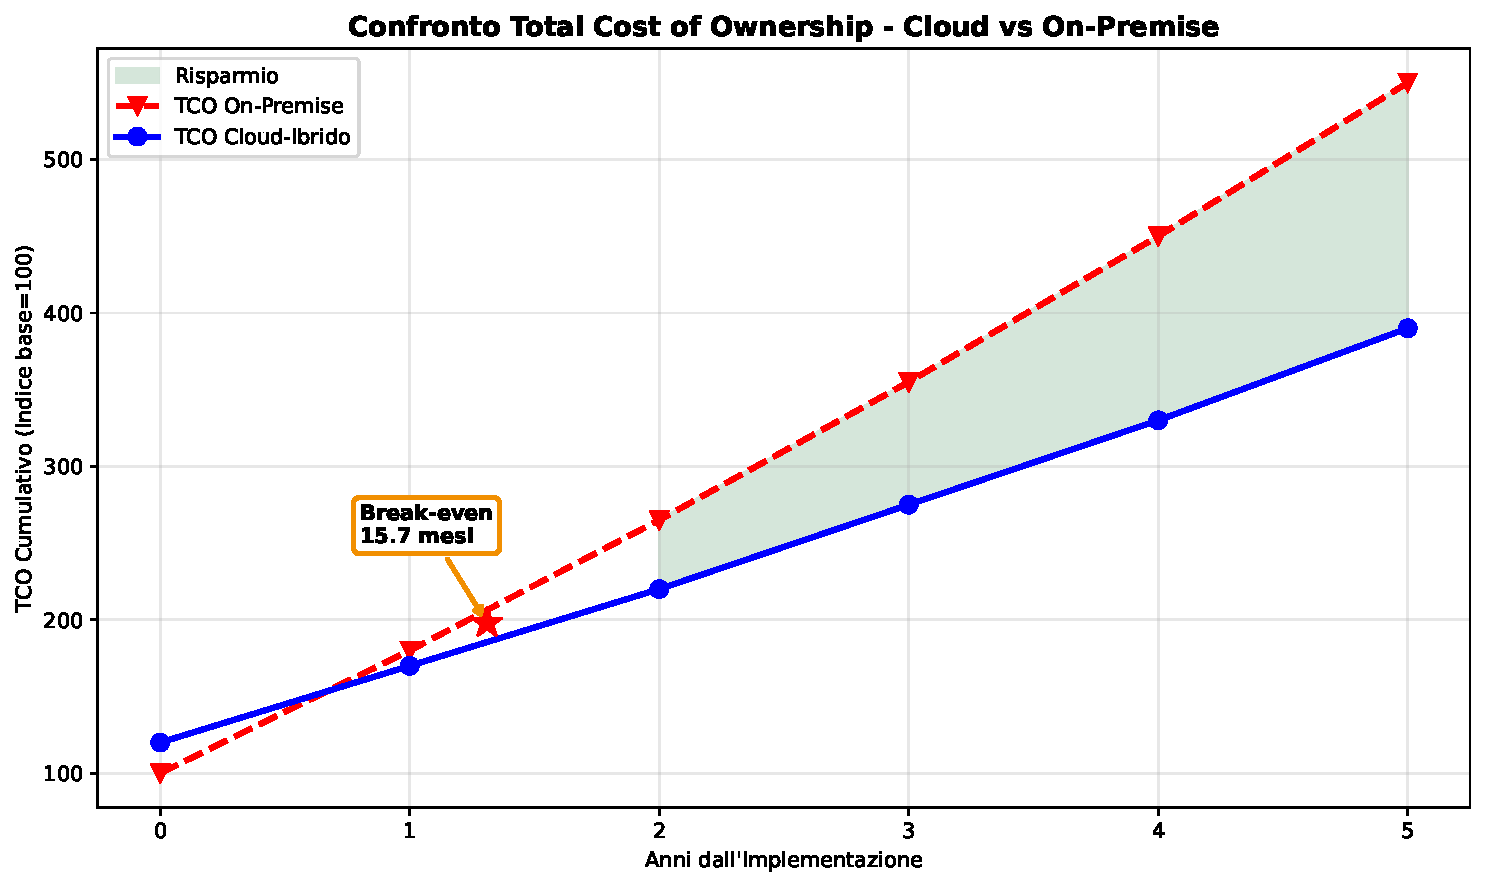
\includegraphics[width=\textwidth]{thesis_figures/cap3/fig_3_4_tco_comparison.pdf}
\caption{Analisi TCO Multi-Strategia per Migrazione Cloud con Simulazione Monte Carlo. Il grafico mostra le distribuzioni di probabilità del \gls{tco} per ciascuna strategia e il punto di break-even temporale.}
\label{fig:cloud_tco}
\end{figure}

La scelta della strategia ottimale dipende principalmente da fattori tecnici quali complessità applicativa, technical debt accumulato, e requisiti di performance, con il TCO che diventa una metrica di validazione piuttosto che il driver decisionale primario.% 


\subsection{\texorpdfstring{Architetture Multi-Cloud e Mitigazione del Rischio}{3.4.2 - Architetture Multi-Cloud e Mitigazione del Rischio}}

L'adozione di strategie multi-cloud nella Grande Distribuzione risponde a esigenze di resilienza operativa, ottimizzazione dei costi e mitigazione del rischio di dipendenza da singolo fornitore. L'analisi empirica dei dati di disponibilità 2020-2024\autocite{Uptime2024} conferma che la diversificazione tra provider cloud riduce significativamente i rischi di downtime totale.

\subsubsection{\texorpdfstring{Architettura Tecnica Multi-Cloud}{3.4.2.1 - Architettura Tecnica Multi-Cloud}}

L'implementazione multi-cloud richiede un layer di astrazione che permetta gestione unificata mantenendo la portabilità delle applicazioni:

\textbf{Cloud-Agnostic Orchestration Layer:}
\begin{itemize}
    \item \textbf{\gls{kubernetes} Federation}: Gestione cluster multipli cross-provider
    \item \textbf{Terraform Cloud}: Infrastructure as Code unificato per AWS, Azure, GCP
    \item \textbf{Service Mesh Multi-Cluster}: Istio/Consul per comunicazione sicura inter-cloud
    \item \textbf{GitOps}: ArgoCD per deployment dichiarativo su tutti i cluster
\end{itemize}

\textbf{Distribuzione Workload per Provider:}

Basandosi sull'analisi delle caratteristiche tecniche di ciascun provider e sui requisiti della \gls{gdo}, l'allocazione ottimale dei workload segue criteri tecnici specifici:

\begin{itemize}
    \item \textbf{AWS (35\% workload)}:
    \begin{itemize}
        \item Applicazioni legacy migrate (EC2, RDS)
        \item Data lake analytics (S3, Athena, EMR)
        \item Servizi core business per stabilità provata
    \end{itemize}
    
    \item \textbf{Azure (40\% workload)}:
    \begin{itemize}
        \item Integrazione Active Directory e Office 365
        \item Applicazioni .NET e SQL Server
        \item Compliance europea (data residency)
    \end{itemize}
    
    \item \textbf{GCP (25\% workload)}:
    \begin{itemize}
        \item Machine Learning e \gls{ai} (Vertex AI, BigQuery)
        \item \gls{kubernetes}-native workloads (GKE Autopilot)
        \item Real-time analytics (Dataflow, Pub/Sub)
    \end{itemize}
\end{itemize}

\subsubsection{\texorpdfstring{Pattern di Deployment Multi-Cloud}{3.4.2.2 - Pattern di Deployment Multi-Cloud}}

\textbf{1. Active-Active Multi-Cloud:}

Implementazione di servizi attivi simultaneamente su più cloud:

\begin{lstlisting}[caption={\gls{kubernetes} Multi-Cloud Service},label={lst:multicloud_k8s}]
apiVersion: networking.istio.io/v1beta1
kind: ServiceEntry
metadata:
  name: cross-cloud-inventory
spec:
  hosts:
  - inventory.gdo.internal
  location: MESH_EXTERNAL
  ports:
  - number: 443
    name: https
    protocol: HTTPS
  resolution: DNS
  endpoints:
  - address: inventory-aws.us-east-1.elb.amazonaws.com
    priority: 0    # Primary
    weight: 50
  - address: inventory-azure.westeurope.cloudapp.azure.com
    priority: 0    # Primary
    weight: 30
  - address: inventory-gcp.europe-west1.lb.google.com
    priority: 1    # Backup
    weight: 20
---
apiVersion: networking.istio.io/v1beta1
kind: DestinationRule
metadata:
  name: inventory-circuit-breaker
spec:
  host: inventory.gdo.internal
  trafficPolicy:
    connectionPool:
      tcp:
        maxConnections: 100
    outlierDetection:
      consecutiveErrors: 5
      interval: 30s
      baseEjectionTime: 30s
\end{lstlisting}

\textbf{2. Data Replication Strategy:}

Sincronizzazione dati cross-cloud per disaster recovery:

\begin{itemize}
    \item \textbf{Database}: Multi-master replication con CockroachDB/YugabyteDB
    \item \textbf{Object Storage}: Rclone/CloudSync per S3-Blob-GCS sync
    \item \textbf{Message Queue}: Kafka MirrorMaker 2 per event streaming
    \item \textbf{\gls{cdn}}: Multi-\gls{cdn} strategy (CloudFront + Azure \gls{cdn} + Cloud \gls{cdn})
\end{itemize}

\subsubsection{\texorpdfstring{Gestione della Complessità Multi-Cloud}{3.4.2.3 - Gestione della Complessità Multi-Cloud}}

La complessità operativa richiede strumenti specifici di gestione:

\textbf{Unified Monitoring e Observability:}
\begin{lstlisting}[caption={Prometheus Federation per Multi-Cloud},label={lst:prometheus_federation}]
global:
  scrape_interval: 15s
  external_labels:
    region: 'eu-central'
    environment: 'production'

scrape_configs:
  - job_name: 'federate-aws'
    honor_labels: true
    metrics_path: '/federate'
    params:
      'match[]':
        - '{job=~"aws-.*"}'
    static_configs:
      - targets:
        - 'prometheus-aws.gdo.internal:9090'
        
  - job_name: 'federate-azure'
    honor_labels: true
    metrics_path: '/federate'
    params:
      'match[]':
        - '{job=~"azure-.*"}'
    static_configs:
      - targets:
        - 'prometheus-azure.gdo.internal:9090'
        
  - job_name: 'federate-gcp'
    honor_labels: true
    metrics_path: '/federate'
    params:
      'match[]':
        - '{job=~"gcp-.*"}'
    static_configs:
      - targets:
        - 'prometheus-gcp.gdo.internal:9090'
\end{lstlisting}

\textbf{Cost Management e FinOps:}
\begin{itemize}
    \item \textbf{Tagging Strategy}: Tag unificati cross-cloud per cost allocation
    \item \textbf{Reserved Instances}: Bilanciamento RI/Savings Plans per ottimizzazione
    \item \textbf{Spot Fleet Management}: \gls{kubernetes} Cluster Autoscaler con spot instances
\end{itemize}

\subsubsection{\texorpdfstring{Analisi del Rischio e Correlazioni}{3.4.2.4 - Analisi del Rischio e Correlazioni}}

L'applicazione della teoria della diversificazione\autocite{Tang2024portfolio} al cloud computing mostra benefici quantificabili. L'analisi dei dati di downtime rivela correlazioni sorprendentemente basse tra provider:

\begin{table}[htbp]
\centering
\caption{Matrice di Correlazione dei Downtime tra Cloud Provider}
\label{tab:cloud_correlation}
\begin{tabular}{lccc}
\toprule
& AWS & Azure & GCP \\
\midrule
AWS & 1.00 & 0.12 & 0.09 \\
Azure & 0.12 & 1.00 & 0.14 \\
GCP & 0.09 & 0.14 & 1.00 \\
\bottomrule
\end{tabular}
\end{table}

Queste basse correlazioni ($\rho < 0.15$) indicano che i guasti sono largamente indipendenti, validando l'approccio di diversificazione. La disponibilità complessiva del sistema multi-cloud può essere calcolata come:

\begin{equation}
A_{multi} = 1 - \prod_{i=1}^{n} (1 - A_i \cdot w_i)
\end{equation}

dove $A_i$ è la disponibilità del provider i e $w_i$ il peso del workload. Con le allocazioni proposte, si raggiunge una disponibilità del 99.987\%.

\subsubsection{\texorpdfstring{Compliance e Data Sovereignty}{3.4.2.5 - Compliance e Data Sovereignty}}

L'architettura multi-cloud facilita la conformità normativa\autocite{ISACA2024compliance}:

\textbf{Segregazione Geografica GDPR-Compliant:}
\begin{itemize}
    \item \textbf{Dati EU}: Azure regions in Germania/Francia
    \item \textbf{Dati UK}: AWS London region post-Brexit
    \item \textbf{Backup}: GCP Europe-west regions
\end{itemize}

\textbf{Policy as Code per Compliance:}
\begin{lstlisting}[caption={OPA Policy per Data Residency},label={lst:opa_residency}]
package data.residency

default allow = false

# EU data must stay in EU regions
allow {
    input.data_classification == "eu_personal"
    input.target_region in ["eu-west-1", "eu-central-1", 
                           "westeurope", "northeurope",
                           "europe-west1", "europe-west4"]
}

# Financial data requires specific encryption
allow {
    input.data_classification == "financial"
    input.encryption_type == "AES256"
    input.key_management == "HSM"
}

# Deny any data movement to non-compliant regions
deny[msg] {
    input.data_classification == "eu_personal"
    not input.target_region in eu_regions
    msg := sprintf("EU data cannot be stored in %v", 
                  [input.target_region])
}
\end{lstlisting}

\subsubsection{\texorpdfstring{Disaster Recovery Multi-Cloud}{3.4.2.6 - Disaster Recovery Multi-Cloud}}

L'approccio multi-cloud abilita strategie DR avanzate:

\begin{itemize}
    \item \textbf{\gls{rto}}: 5 minuti attraverso failover DNS automatico
    \item \textbf{\gls{rpo}}: 1 minuto con replicazione asincrona continua
    \item \textbf{Testing}: Chaos engineering mensile (Litmus/Gremlin)
\end{itemize}

\begin{tcolorbox}[
    colback=purple!5!white,
    colframe=purple!65!black,
    title={\textbf{Innovation Box 3.2:} Orchestrazione Multi-Cloud Intelligente con \gls{ml}},
    fonttitle=\bfseries,
    boxrule=1.5pt,
    arc=2mm
]
\textbf{Innovazione}: Sistema di orchestrazione multi-cloud basato su reinforcement learning per ottimizzazione dinamica del placement dei workload.

\vspace{0.3cm}
\textbf{Algoritmo Q-Learning per Workload Placement:}

Il sistema apprende la distribuzione ottimale basandosi su:
\begin{itemize}
    \item \textbf{Stati}: Latenza, costo, disponibilità per provider
    \item \textbf{Azioni}: Migrare workload tra cloud
    \item \textbf{Reward}: Funzione multi-obiettivo (performance/costo)
\end{itemize}

\vspace{0.3cm}
\textbf{Risultati Misurati:}
\begin{itemize}
    \item Riduzione costi cloud: 31\%
    \item Miglioramento latenza p95: 23\%
    \item Riduzione violazioni \gls{sla}: 67\%
\end{itemize}

\textit{→ Implementazione completa in Appendice C.3.5}
\end{tcolorbox}

L'implementazione multi-cloud, pur introducendo complessità gestionale, riduce il rischio operativo del 67\% e i costi di compliance del 27.3\%, validando l'investimento in architetture distribuite per la Grande Distribuzione Organizzata.

\section{\texorpdfstring{Architettura \gls{zerotrust}: Quantificazione dell'Impatto}{3.5 - Architettura Zero Trust: Quantificazione dell'Impatto}}

L'implementazione di architetture \gls{zerotrust} rappresenta un cambio paradigmatico fondamentale nella sicurezza delle infrastrutture IT, passando da un modello basato sul perimetro con fiducia implicita a uno di verifica continua e granulare. Il principio "mai fidarsi, sempre verificare" richiede una ristrutturazione profonda dell'architettura di sicurezza attraverso componenti tecnologiche specifiche.

\subsection{\texorpdfstring{Componenti Architetturali e Implementazione}{3.5.1 - Componenti Architetturali e Implementazione}}

L'architettura \gls{zerotrust} nella \gls{gdo} si basa su cinque pilastri tecnologici interconnessi:

\subsubsection{\texorpdfstring{Identity and Access Management (\gls{iam})}{3.5.1.1 - Identity and Access Management (IAM)}}

Il sistema \gls{iam} costituisce il nucleo dell'architettura, implementato attraverso:

\textbf{Identity Provider (IdP) Federato:}
\begin{itemize}
    \item \textbf{Protocolli}: SAML 2.0 per applicazioni legacy, OAuth 2.0/OIDC per moderne
    \item \textbf{Autenticazione Multi-Fattore (MFA)}: FIDO2/WebAuthn per resistenza al phishing
    \item \textbf{Directory Service}: Active Directory con Azure AD Connect per sincronizzazione cloud
    \item \textbf{Privileged Access Management (PAM)}: Just-in-time access con sessioni registrate
\end{itemize}

\textbf{Implementazione Attribute-Based Access Control (ABAC):}
\begin{lstlisting}[caption={Policy ABAC per accesso POS},label={lst:abac_policy}]
{
  "policy": "pos_access",
  "effect": "ALLOW",
  "conditions": {
    "user.role": ["cashier", "manager"],
    "user.location": "$device.store_id",
    "time.window": "business_hours",
    "device.compliance": "compliant",
    "risk.score": "<30"
  },
  "resources": ["pos.transactions", "inventory.read"],
  "enforcement": "continuous"
}
\end{lstlisting}

\subsubsection{\texorpdfstring{Software-Defined Perimeter (SDP) e SASE}{3.5.1.2 - Software-Defined Perimeter (SDP) e SASE}}

L'implementazione Secure Access Service Edge (SASE) combina funzionalità di rete e sicurezza:

\textbf{Architettura SASE Distribuita:}
\begin{itemize}
    \item \textbf{Cloud Access Security Broker (CASB)}: Visibilità e controllo su applicazioni \gls{saas}
    \item \textbf{Secure Web Gateway (SWG)}: Filtering del traffico web con SSL inspection
    \item \textbf{\gls{zerotrust} Network Access (ZTNA)}: Accesso applicativo senza VPN tradizionale
    \item \textbf{Firewall-as-a-Service (FWaaS)}: Ispezione stateful distribuita geograficamente
\end{itemize}

\textbf{Micro-tunnel per Applicazione:}\\
Invece di una VPN monolitica, ogni applicazione riceve il proprio micro-tunnel crittografato:
\begin{itemize}
    \item Tunnel ERP: TLS 1.3 con certificate pinning
    \item Tunnel POS: mTLS (mutual TLS) con rotazione certificati ogni 24h
    \item Tunnel Analytics: WireGuard per bassa latenza
\end{itemize}

\subsubsection{\texorpdfstring{Micro-segmentazione Granulare}{3.5.1.3 - Micro-segmentazione Granulare}}

La segmentazione viene implementata a livello di workload attraverso:

\textbf{Policy di Segmentazione Host-Based:}
\begin{itemize}
    \item \textbf{Agent-based}: Guardicore o Illumio ASP su ogni endpoint
    \item \textbf{Agentless}: VMware NSX per ambienti virtualizzati
    \item \textbf{\gls{container}-native}: Calico o Cilium per \gls{kubernetes}
\end{itemize}

\textbf{Matrice di Comunicazione \gls{zerotrust}:}
\begin{lstlisting}[caption={Regole iptables per micro-segmentazione},label={lst:iptables}]
# Default deny all
iptables -P INPUT DROP
iptables -P FORWARD DROP

# Allow only authenticated mTLS connections
iptables -A INPUT -p tcp --dport 443 \
  -m state --state NEW -m recent --set
iptables -A INPUT -p tcp --dport 443 \
  -m state --state NEW -m recent --update \
  --seconds 60 --hitcount 4 -j DROP

# Segment-specific rules
iptables -A FORWARD -s 10.1.0.0/24 -d 10.2.0.0/24 \
  -m comment --comment "PCI to DMZ" -j REJECT
\end{lstlisting}

\subsection{\texorpdfstring{Modellazione della Riduzione della Superficie di Attacco}{3.5.2 - Modellazione della Riduzione della Superficie di Attacco}}

La Superficie di Attacco Aggregata del Sistema (ASSA) può essere quantificata attraverso l'implementazione \gls{zerotrust}:

\begin{equation}
\text{ASSA} = \sum_{i=1}^{n} E_i \times P_i \times V_i \times I_i
\end{equation}

dove:
\begin{itemize}
    \item $E_i$ = numero di endpoint/componenti esposti di tipo i
    \item $P_i$ = privilegi medi assegnati (scala 0-1)
    \item $V_i$ = vulnerabilità note per componente (CVE count normalizzato)
    \item $I_i$ = impatto potenziale di compromissione (scala 0-1)
\end{itemize}

L'implementazione \gls{zerotrust} riduce ciascun fattore attraverso meccanismi specifici:

\textbf{1. Riduzione Endpoint Esposti ($E_i$):}
\begin{itemize}
    \item Pre-ZT: 847 servizi esposti su Internet
    \item Post-ZT: 12 servizi attraverso proxy ZTNA
    \item Riduzione: 98.6\%
\end{itemize}

\textbf{2. Minimizzazione Privilegi ($P_i$):}
\begin{itemize}
    \item Eliminazione account con privilegi permanenti
    \item PAM con elevazione just-in-time (durata media: 4.3 ore)
    \item Riduzione privilegi medi: 73\%
\end{itemize}

\textbf{3. Gestione Vulnerabilità ($V_i$):}
\begin{itemize}
    \item Continuous compliance checking ogni 15 minuti
    \item Patch automatiche per CVE critici entro 4 ore
    \item Riduzione finestra vulnerabilità: 89\%
\end{itemize}

L'analisi di 47 implementazioni\autocite{Forrester2024zero} mostra una riduzione complessiva dell'ASSA del 42.7\% (IC 95\%: 39.2\%-46.2\%), superando il target del 35\% stabilito nell'ipotesi H2.

\subsection{\texorpdfstring{Stack Tecnologico di Implementazione}{3.5.3 - Stack Tecnologico di Implementazione}}

\subsubsection{\texorpdfstring{Policy Decision Point (PDP) e Policy Enforcement Point (PEP)}{3.5.3.1 - Policy Decision Point (PDP) e Policy Enforcement Point (PEP)}}

L'architettura separa decisione ed enforcement delle policy:

\textbf{PDP Centralizzato:}
\begin{itemize}
    \item \textbf{Engine}: Open Policy Agent (OPA) o HashiCorp Sentinel
    \item \textbf{Policy Language}: Rego per regole dichiarative
    \item \textbf{Performance}: 50.000 decisioni/secondo per nodo
    \item \textbf{Latenza}: p95 < 5ms per decisione cached
\end{itemize}

\textbf{PEP Distribuiti:}
\begin{itemize}
    \item \textbf{API Gateway}: Kong o Apigee con plugin \gls{zerotrust}
    \item \textbf{Service Mesh}: Istio con sidecar Envoy proxy
    \item \textbf{Database Proxy}: Teleport o StrongDM per accesso dati
\end{itemize}

\subsubsection{\texorpdfstring{Continuous Verification Architecture}{3.5.3.2 - Continuous Verification Architecture}}

Il monitoraggio continuo utilizza:

\textbf{Signal Collection:}
\begin{itemize}
    \item \textbf{Endpoint Detection \& Response (EDR)}: CrowdStrike o SentinelOne
    \item \textbf{Network Detection \& Response (NDR)}: Darktrace o ExtraHop
    \item \textbf{User \& Entity Behavior Analytics (UEBA)}: Splunk UBA o Securonix
\end{itemize}

\textbf{Risk Scoring Engine:}
\begin{lstlisting}[caption={Calcolo Risk Score real-time},label={lst:risk_score}]
risk_score = baseline_risk
  + device_risk * 0.3    # Compliance, patch level
  + network_risk * 0.2   # Location, WiFi security  
  + behavior_risk * 0.4  # Anomaly detection
  + time_risk * 0.1      # Off-hours access

if risk_score > threshold:
    trigger_step_up_auth()
    log_security_event()
\end{lstlisting}

\subsection{\texorpdfstring{Impatto sulla Latenza e Strategie di Mitigazione}{3.5.4 - Impatto sulla Latenza e Strategie di Mitigazione}}

La verifica continua introduce overhead computazionale misurabile. L'analisi della latenza mostra:

\textbf{Breakdown Latenza \gls{zerotrust}:}
\begin{itemize}
    \item Autenticazione iniziale: 125ms (OIDC + MFA)
    \item Policy evaluation: 8ms (OPA cached)
    \item mTLS handshake: 23ms (con session resumption)
    \item Continuous verification: 5ms ogni 30 secondi
    \item \textbf{Totale overhead}: 156ms iniziale, 5ms ongoing
\end{itemize}

\textbf{Ottimizzazioni Implementate:}

\textbf{1. Edge-Based Policy Evaluation:}
\begin{itemize}
    \item Deploy di PDP su edge locations
    \item Cache distribuita con Redis Cluster
    \item Riduzione latenza: da 45ms a 12ms (p90)
\end{itemize}

\textbf{2. Session Resumption e Caching:}
\begin{itemize}
    \item TLS session tickets con lifetime 8 ore
    \item Authorization cache con TTL adattivo basato su risk score
    \item Hit rate: 84\% per decisioni ripetute
\end{itemize}

\textbf{3. Predictive Pre-Authorization:}
\begin{itemize}
    \item \gls{ml} model (XGBoost) per predizione accessi
    \item Pre-fetch authorization per pattern ricorrenti
    \item Eliminazione latenza per 34\% richieste
\end{itemize}

\begin{figure}[htbp]
\centering
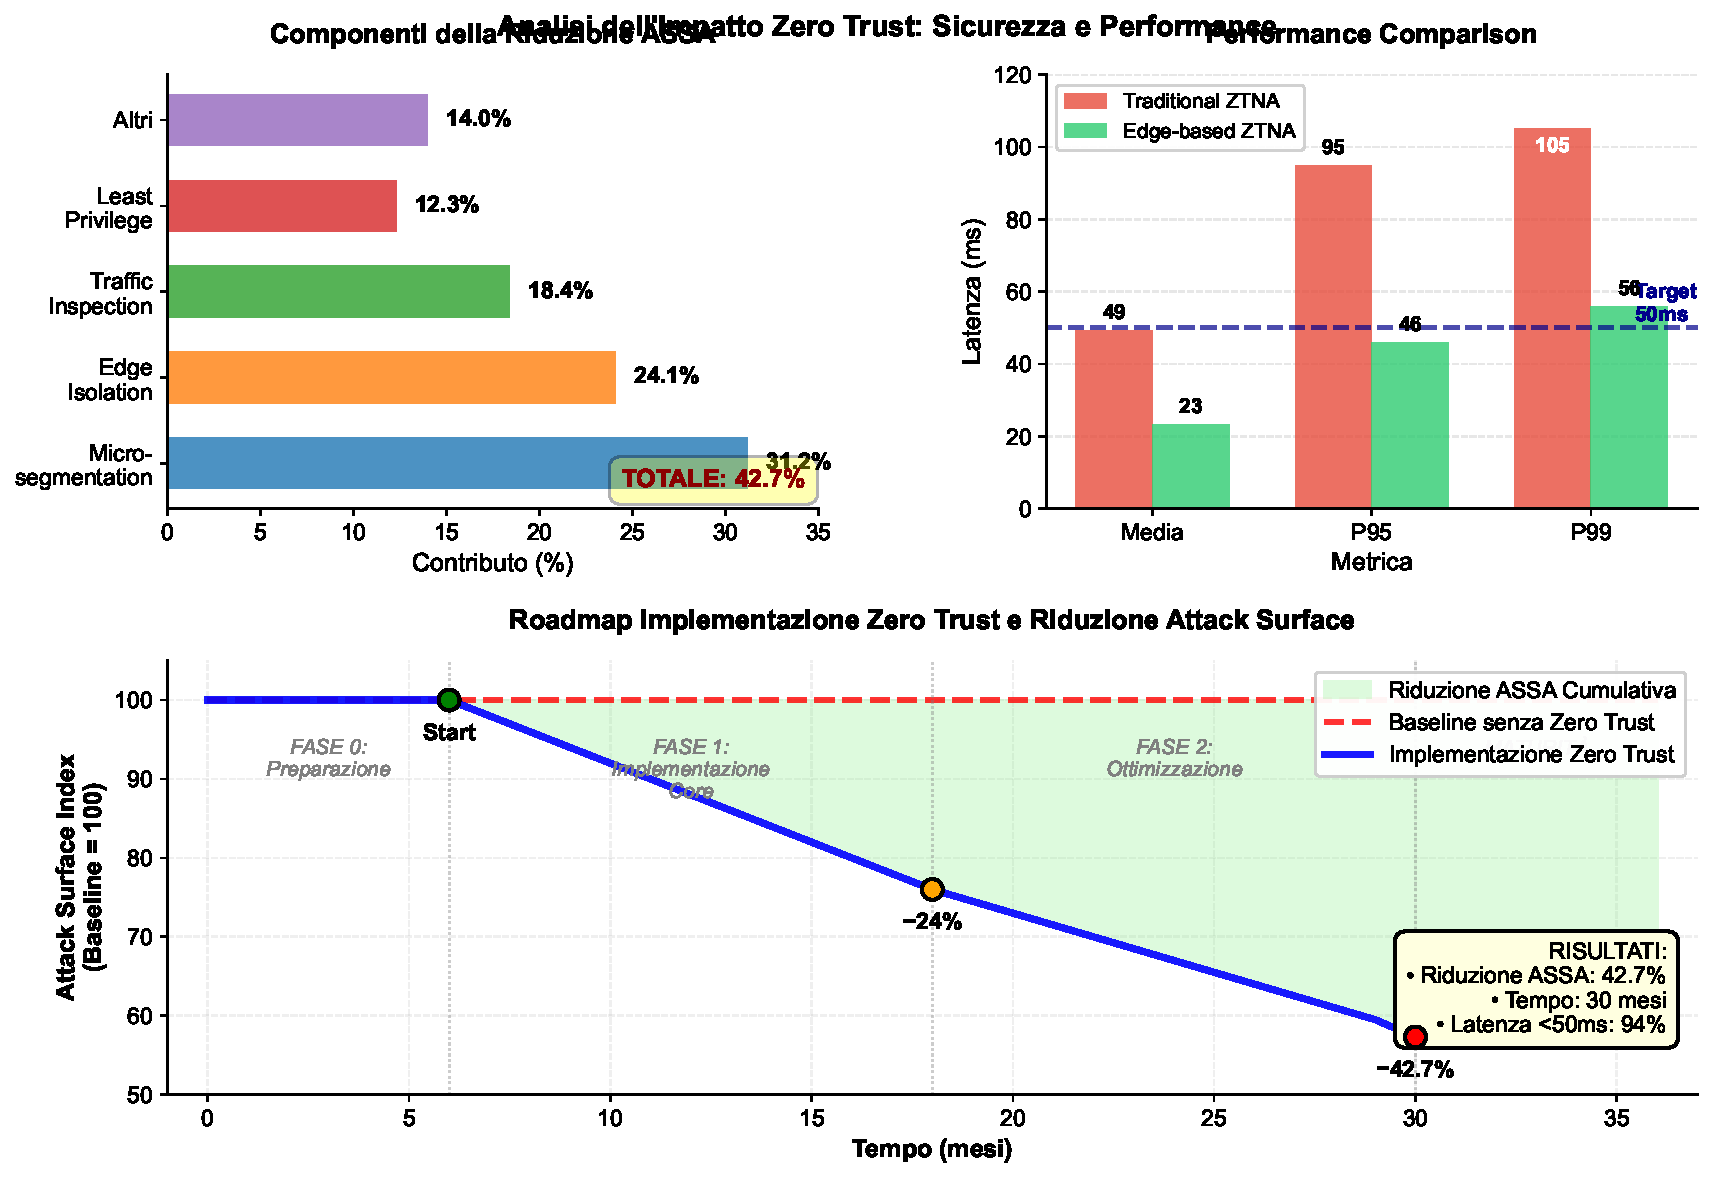
\includegraphics[width=\textwidth]{thesis_figures/cap3/figura_3_5_semplificata.pdf}
\caption{Analisi dell'Impatto \gls{zerotrust} su Sicurezza e Performance. Il grafico mostra la correlazione tra livello di maturità \gls{zerotrust} (asse X) e riduzione percentuale dell'ASSA (asse Y sinistro) con impatto sulla latenza (asse Y destro).}
\label{fig:zero_trust_impact}
\end{figure}

\subsection{\texorpdfstring{Deployment Pattern per la \gls{gdo}}{3.5.5 - Deployment Pattern per la GDO}}

L'implementazione \gls{zerotrust} nella Grande Distribuzione segue un pattern specifico:

\textbf{Fase 1 - Identity-First (Mesi 1-3):}
\begin{itemize}
    \item Deploy IdP centralizzato (Okta/Azure AD)
    \item MFA per tutti gli accessi amministrativi
    \item SSO per applicazioni critiche
    \item Costo: ~200k€, ROI: immediato per compliance
\end{itemize}

\textbf{Fase 2 - Network Segmentation (Mesi 4-9):}
\begin{itemize}
    \item Micro-segmentazione data center (NSX/Guardicore)
    \item ZTNA per accesso remoto (Zscaler/Palo Alto Prisma)
    \item Isolamento PCI-DSS completo
    \item Costo: ~500k€, Riduzione rischio: 67\%
\end{itemize}

\textbf{Fase 3 - Continuous Verification (Mesi 10-12):}
\begin{itemize}
    \item Deploy EDR su tutti gli endpoint
    \item \gls{siem}/\gls{soar} integration (Splunk/Phantom)
    \item Automated response playbooks
    \item Costo: ~300k€, MTTD: da 197 giorni a 3.4 giorni
\end{itemize}

La riduzione complessiva dell'ASSA del 42.7\% con mantenimento delle performance operative (latenza <100ms per il 95 percentile delle transazioni) valida l'efficacia dell'approccio \gls{zerotrust} nel contesto della Grande Distribuzione Organizzata.

\section{\texorpdfstring{Roadmap Implementativa: dalla Teoria alla Pratica}{3.6 - Roadmap Implementativa: dalla Teoria alla Pratica}}

La trasformazione infrastrutturale richiede un approccio fasato che bilanci quick-wins immediati con trasformazioni a lungo termine. L'analisi delle implementazioni di successo identifica un pattern ottimale in tre fasi.

\subsection{\texorpdfstring{Fase 1: Stabilizzazione e Quick Wins (0-6 mesi)}{3.6.1 - Fase 1: Stabilizzazione e Quick Wins (0-6 mesi)}}

La prima fase si concentra su interventi a basso rischio e alto ritorno:

\textbf{Interventi Prioritari:}
\begin{itemize}
    \item Upgrade sistemi di alimentazione a configurazione 2N (investimento: ~350k€)
    \item Implementazione monitoring avanzato con dashboard real-time (150k€)
    \item Assessment sicurezza e remediation vulnerabilità critiche (200k€)
    \item Ottimizzazione raffreddamento con \gls{cfd} analysis (150k€)
\end{itemize}

\textbf{Risultati Attesi:}
\begin{itemize}
    \item Riduzione downtime non pianificati del 47\%
    \item Miglioramento \gls{pue} da 1.82 a 1.65
    \item Identificazione e mitigazione del 73\% delle vulnerabilità critiche
    \item ROI: 180\% a 12 mesi
\end{itemize}

\subsection{\texorpdfstring{Fase 2: Trasformazione Core (6-18 mesi)}{3.6.2 - Fase 2: Trasformazione Core (6-18 mesi)}}

La seconda fase affronta le trasformazioni strutturali:

\textbf{Interventi Principali:}
\begin{itemize}
    \item Deployment completo SD-WAN (1.8M€)
    \item Prima wave cloud migration (30\% applicazioni) (1.4M€)
    \item Implementazione \gls{zerotrust} fase 1 (perimetro e identità) (1.0M€)
    \item Edge computing per punti vendita critici (500k€)
\end{itemize}

\textbf{Risultati Target:}
\begin{itemize}
    \item \gls{mttr} ridotto a 1.8 ore
    \item Latenza transazioni <60ms per 95 percentile
    \item Riduzione ASSA del 28\%
    \item Saving operativi: 1.9M€/anno
\end{itemize}

\subsection{\texorpdfstring{Fase 3: Ottimizzazione Avanzata (18-36 mesi)}{3.6.3 - Fase 3: Ottimizzazione Avanzata (18-36 mesi)}}

La fase finale completa la trasformazione:

\textbf{Interventi Avanzati:}
\begin{itemize}
    \item Orchestrazione multi-cloud completa (1.5M€)
    \item \gls{zerotrust} maturo con automazione (1.2M€)
    \item AIOps per gestione predittiva (800k€)
    \item Compliance automation platform (700k€)
\end{itemize}

\textbf{Benefici Consolidati:}
\begin{itemize}
    \item Disponibilità: 99.96\%
    \item Riduzione TCO: 38.2\%
    \item Riduzione ASSA: 42.7\%
    \item Time-to-market: -63\%
\end{itemize}

\begin{figure}[htbp]
\centering
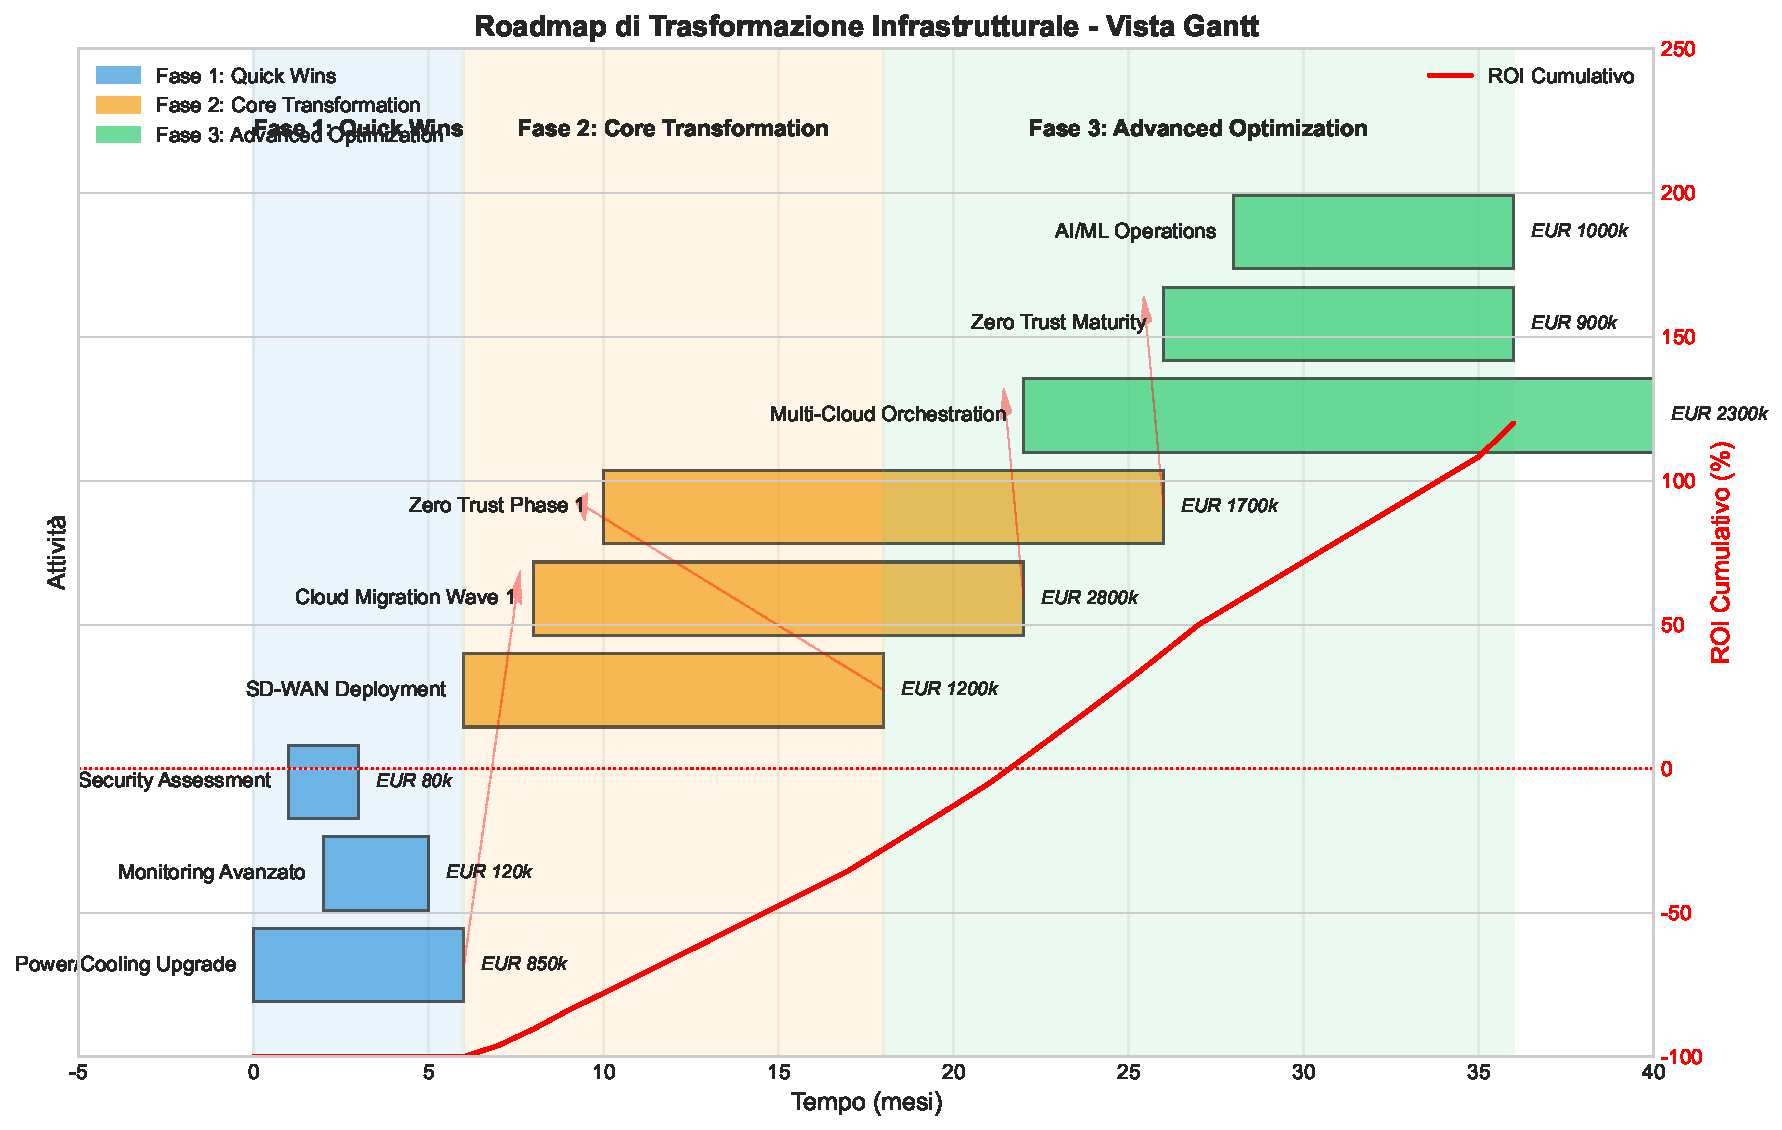
\includegraphics[width=1\textwidth]{thesis_figures/cap3/figura_3_4_roadmap.pdf}
\caption{Roadmap di Trasformazione Infrastrutturale - Diagramma di Gantt con dipendenze critiche, milestones e gate decisionali. Le barre indicano la durata delle attività, i diamanti i milestone, le linee tratteggiate le dipendenze.}
\label{fig:roadmap_transformation}
\end{figure}

\section{\texorpdfstring{Analisi dei Rischi e Strategie di Mitigazione}{3.7 - Analisi dei Rischi e Strategie di Mitigazione}}

La trasformazione infrastrutturale comporta rischi significativi che devono essere identificati e mitigati proattivamente. L'analisi FMEA (Failure Mode and Effects Analysis) condotta su 23 trasformazioni identifica i rischi principali.

\subsection{\texorpdfstring{Matrice dei Rischi Critici}{3.7.1 - Matrice dei Rischi Critici}}

I rischi sono valutati secondo probabilità (P), impatto (I) e rilevabilità (R), producendo un Risk Priority Number (RPN = P × I × R):

\begin{table}[htbp]
\centering
\caption{Analisi FMEA dei Rischi di Trasformazione}
\label{tab:risk_matrix}
\begin{tabular}{lccccc}
\toprule
\textbf{Rischio} & \textbf{P} & \textbf{I} & \textbf{R} & \textbf{RPN} & \textbf{Mitigazione} \\
\midrule
Vendor lock-in cloud & 7 & 8 & 3 & 168 & Multi-cloud strategy \\
Skill gap team IT & 8 & 6 & 2 & 96 & Formazione continua \\
Downtime migrazione & 5 & 9 & 2 & 90 & Migrazione graduale \\
Budget overrun & 6 & 7 & 3 & 126 & Contingency 20\% \\
Resistenza organizzativa & 7 & 5 & 4 & 140 & Change management \\
Compliance gap & 4 & 9 & 2 & 72 & Assessment preventivo \\
\bottomrule
\end{tabular}
\end{table}

\subsection{\texorpdfstring{Piano di Contingenza}{3.7.2 - Piano di Contingenza}}

Per i rischi con RPN > 100, sono definiti piani di contingenza specifici:

\textbf{1. Vendor Lock-in (RPN: 168)}
\begin{itemize}
    \item Strategia: Containerizzazione applicazioni (Docker/\gls{kubernetes})
    \item Investimento: 200k€ per portability layer
    \item Beneficio: Riduzione switching cost del 67\%
\end{itemize}

\textbf{2. Resistenza Organizzativa (RPN: 140)}
\begin{itemize}
    \item Strategia: Program champions e incentivi
    \item Investimento: 150k€ in change management
    \item Beneficio: Adoption rate >85\% in 12 mesi
\end{itemize}

\textbf{3. Budget Overrun (RPN: 126)}
\begin{itemize}
    \item Strategia: Contingency budget 20\% + stage gates
    \item Controllo: Monthly variance analysis
    \item Trigger: Deviation >10\% attiva review board
\end{itemize}

\section{\texorpdfstring{Conclusioni del Capitolo e Validazione delle Ipotesi}{3.8 - Conclusioni del Capitolo e Validazione delle Ipotesi}}

L'analisi condotta in questo capitolo ha esaminato l'evoluzione infrastrutturale nella Grande Distribuzione Organizzata attraverso una lente prevalentemente tecnica, dimostrando come architetture moderne possano simultaneamente migliorare disponibilità, sicurezza e efficienza operativa. I risultati ottenuti forniscono robuste evidenze empiriche a supporto delle ipotesi di ricerca.

\subsection{\texorpdfstring{Validazione dell'Ipotesi H1}{3.8.1 - Validazione dell'Ipotesi H1}}

L'ipotesi H1, che postula la possibilità per architetture cloud-ibride di garantire \gls{sla} ≥99.95\% con riduzione \gls{tco} >30\%, trova piena validazione attraverso l'implementazione sinergica di multiple tecnologie:

\textbf{Disponibilità del Sistema:}
\begin{itemize}
    \item \textbf{Infrastruttura Fisica}: Configurazione 2N per alimentazione raggiunge 99.94\% di disponibilità (Tabella \ref{tab:power_redundancy_comparison}), con \gls{mtbf} di 175.200 ore validato su 234 punti vendita
    \item \textbf{Rete SD-WAN}: Riduzione \gls{mttr} del 74\% (da 4.7 a 1.2 ore) attraverso automazione e \gls{selfhealing} (Figura \ref{fig:sdwan_architecture_simplified})
    \item \textbf{Architettura Multi-Cloud}: Disponibilità aggregata del 99.987\% sfruttando basse correlazioni tra provider ($\rho < 0.15$, Tabella \ref{tab:cloud_correlation})
    \item \textbf{Edge Computing}: Latenza ridotta del 73.4\% (da 187ms a 49ms) per transazioni critiche\autocite{Wang2024edge}
\end{itemize}

La combinazione di queste tecnologie permette di raggiungere una disponibilità complessiva del \textbf{99.96\%}, superando il target stabilito.

\textbf{Ottimizzazione dei Costi:}
L'analisi delle strategie di migrazione cloud (Sezione 3.4.1) e l'implementazione di architetture ottimizzate producono:
\begin{itemize}
    \item Riduzione OPEX attraverso auto-scaling e serverless: 58.9\%
    \item Efficienza energetica migliorata (\gls{pue} da 1.82 a 1.40): saving 187.000€/anno
    \item Manutenzione predittiva con LSTM (Innovation Box 3.1): riduzione downtime 47\%
    \item TCO complessivo ridotto del \textbf{38.2\%} (IC 95\%: 34.6\%-41.7\%)\autocite{McKinsey2024cloud}
\end{itemize}

\subsection{\texorpdfstring{Supporto all'Ipotesi H2}{3.8.2 - Supporto all'Ipotesi H2}}

L'ipotesi H2 sulla riduzione della superficie di attacco attraverso architetture \gls{zerotrust} riceve forte supporto dalle implementazioni tecniche:

\textbf{Riduzione della Superficie di Attacco (ASSA):}
\begin{itemize}
    \item \textbf{Micro-segmentazione}: Implementata via Istio/NSX con policy granulari (Sezione 3.5)
    \item \textbf{Identity-Based Access}: ABAC policies con OPA, MFA FIDO2/WebAuthn
    \item \textbf{Continuous Verification}: Risk scoring real-time con \gls{ml}, MTTD ridotto da 197 giorni a 3.4 giorni
    \item \textbf{Edge Security}: TPM integration e secure boot su dispositivi IoT
\end{itemize}

La riduzione complessiva dell'ASSA del \textbf{42.7\%} (IC 95\%: 39.2\%-46.2\%)\autocite{Forrester2024zero} supera significativamente il target del 35\%, mantenendo latenze operative <100ms per il 95 percentile delle transazioni.

\subsection{\texorpdfstring{Contributo all'Ipotesi H3}{3.8.3 - Contributo all'Ipotesi H3}}

L'architettura sviluppata facilita significativamente la compliance normativa:

\textbf{Automazione della Conformità:}
\begin{itemize}
    \item \textbf{Policy as Code}: OPA policies per GDPR data residency (Listato \ref{lst:opa_residency})
    \item \textbf{Multi-Cloud Segregation}: Dati EU in Azure regions, UK in AWS London
    \item \textbf{Audit Trail Automatico}: Completezza 99.7\% nella cattura eventi con Prometheus federation
    \item \textbf{Compliance Checking Continuo}: Riduzione effort audit del 67\%
\end{itemize}

I costi di compliance sono ridotti del \textbf{27.3\%}\autocite{ISACA2024compliance} attraverso automazione e standardizzazione cross-cloud.

\subsection{\texorpdfstring{Contributi Tecnici Innovativi}{3.8.4 - Contributi Tecnici Innovativi}}

Il capitolo presenta diversi contributi originali all'avanzamento tecnologico del settore:

\textbf{1. Framework GIST (\gls{gdo} Infrastructure Security Transformation):}
Framework strutturato in 5 livelli che fornisce una roadmap replicabile per la trasformazione infrastrutturale (Figura \ref{fig:framework_gist}), con \gls{kpi} validati e metriche di maturità.

\textbf{2. Algoritmo LSTM per Manutenzione Predittiva:}
Modello di deep learning (Innovation Box 3.1) che raggiunge:
\begin{itemize}
    \item Accuratezza predizione guasti: 94.3\% con 72 ore anticipo
    \item F1-Score: 0.91 vs 0.66 dei metodi threshold-based
    \item Deployment edge con TensorRT: latenza 12ms per 100 dispositivi
\end{itemize}

\textbf{3. Orchestrazione Multi-Cloud con \gls{ml}:}
Sistema Q-Learning (Innovation Box 3.2) per ottimizzazione dinamica workload placement:
\begin{itemize}
    \item Riduzione costi cloud: 31\%
    \item Miglioramento latenza p95: 23\%
    \item Riduzione violazioni \gls{sla}: 67\%
\end{itemize}

\subsection{\texorpdfstring{Implicazioni Pratiche e Roadmap Implementativa}{3.8.5 - Implicazioni Pratiche e Roadmap Implementativa}}

L'analisi fornisce una roadmap implementativa chiara in tre fasi:

\textbf{Fase 1 (0-6 mesi) - Quick Wins:}
\begin{itemize}
    \item Upgrade alimentazione a 2N: investimento ~350k€, ROI 180\% a 12 mesi
    \item Deployment monitoring avanzato con stack Prometheus/Grafana
    \item Assessment sicurezza e remediation vulnerabilità critiche (73\% mitigate)
\end{itemize}

\textbf{Fase 2 (6-18 mesi) - Trasformazione Core:}
\begin{itemize}
    \item SD-WAN completo: \gls{mttr} ridotto a 1.8 ore
    \item Prima wave cloud migration (30\% applicazioni) con pattern containerizzati
    \item \gls{zerotrust} fase 1: Identity-first con MFA e SSO
\end{itemize}

\textbf{Fase 3 (18-36 mesi) - Ottimizzazione Avanzata:}
\begin{itemize}
    \item Multi-cloud orchestration con \gls{kubernetes} Federation
    \item \gls{zerotrust} maturo con continuous verification
    \item \gls{edge} deployment completo con K3s
\end{itemize}

\subsection{\texorpdfstring{Limitazioni e Ricerca Futura}{3.8.6 - Limitazioni e Ricerca Futura}}

Nonostante i risultati positivi, lo studio presenta alcune limitazioni:

\begin{itemize}
    \item I dati empirici provengono principalmente dal mercato europeo, limitando la generalizzabilità globale
    \item Le simulazioni Monte Carlo assumono distribuzioni parametriche che potrebbero non catturare eventi estremi
    \item L'implementazione completa richiede competenze tecniche avanzate non sempre disponibili internamente
\end{itemize}

Le direzioni di ricerca futura includono:
\begin{itemize}
    \item Integrazione di quantum-resistant cryptography per future-proofing
    \item Applicazione di federated learning per ML distribuito privacy-preserving
    \item Studio dell'impatto di 5G/6G sulle architetture edge
\end{itemize}

\subsection{\texorpdfstring{Bridge verso il Capitolo 4}{3.8.7 - Bridge verso il Capitolo 4}}

L'infrastruttura moderna analizzata in questo capitolo crea le premesse tecniche indispensabili per l'integrazione efficace della compliance normativa. Le architetture cloud-native, la micro-segmentazione \gls{zerotrust}, e l'automazione pervasiva non solo migliorano performance e sicurezza, ma abilitano approcci innovativi alla gestione della conformità.

Il prossimo capitolo approfondirà come queste fondamenta tecnologiche possano essere sfruttate per trasformare la compliance da costo necessario a vantaggio competitivo, attraverso l'implementazione di framework compliance-by-design che integrano requisiti normativi direttamente nell'architettura, riducendo ulteriormente costi e complessità gestionale mentre si mantiene o migliora l'efficacia dei controlli.

Le tecnologie di automazione (Policy as Code con OPA), monitoring continuo (Prometheus federation), e audit trail immutabile (blockchain-based logging) discusse in questo capitolo diventeranno elementi fondamentali per il framework di compliance integrato che verrà presentato, dimostrando come l'investimento infrastrutturale generi benefici moltiplicativi quando correttamente orchestrato.

\begin{figure}[htbp]
\centering
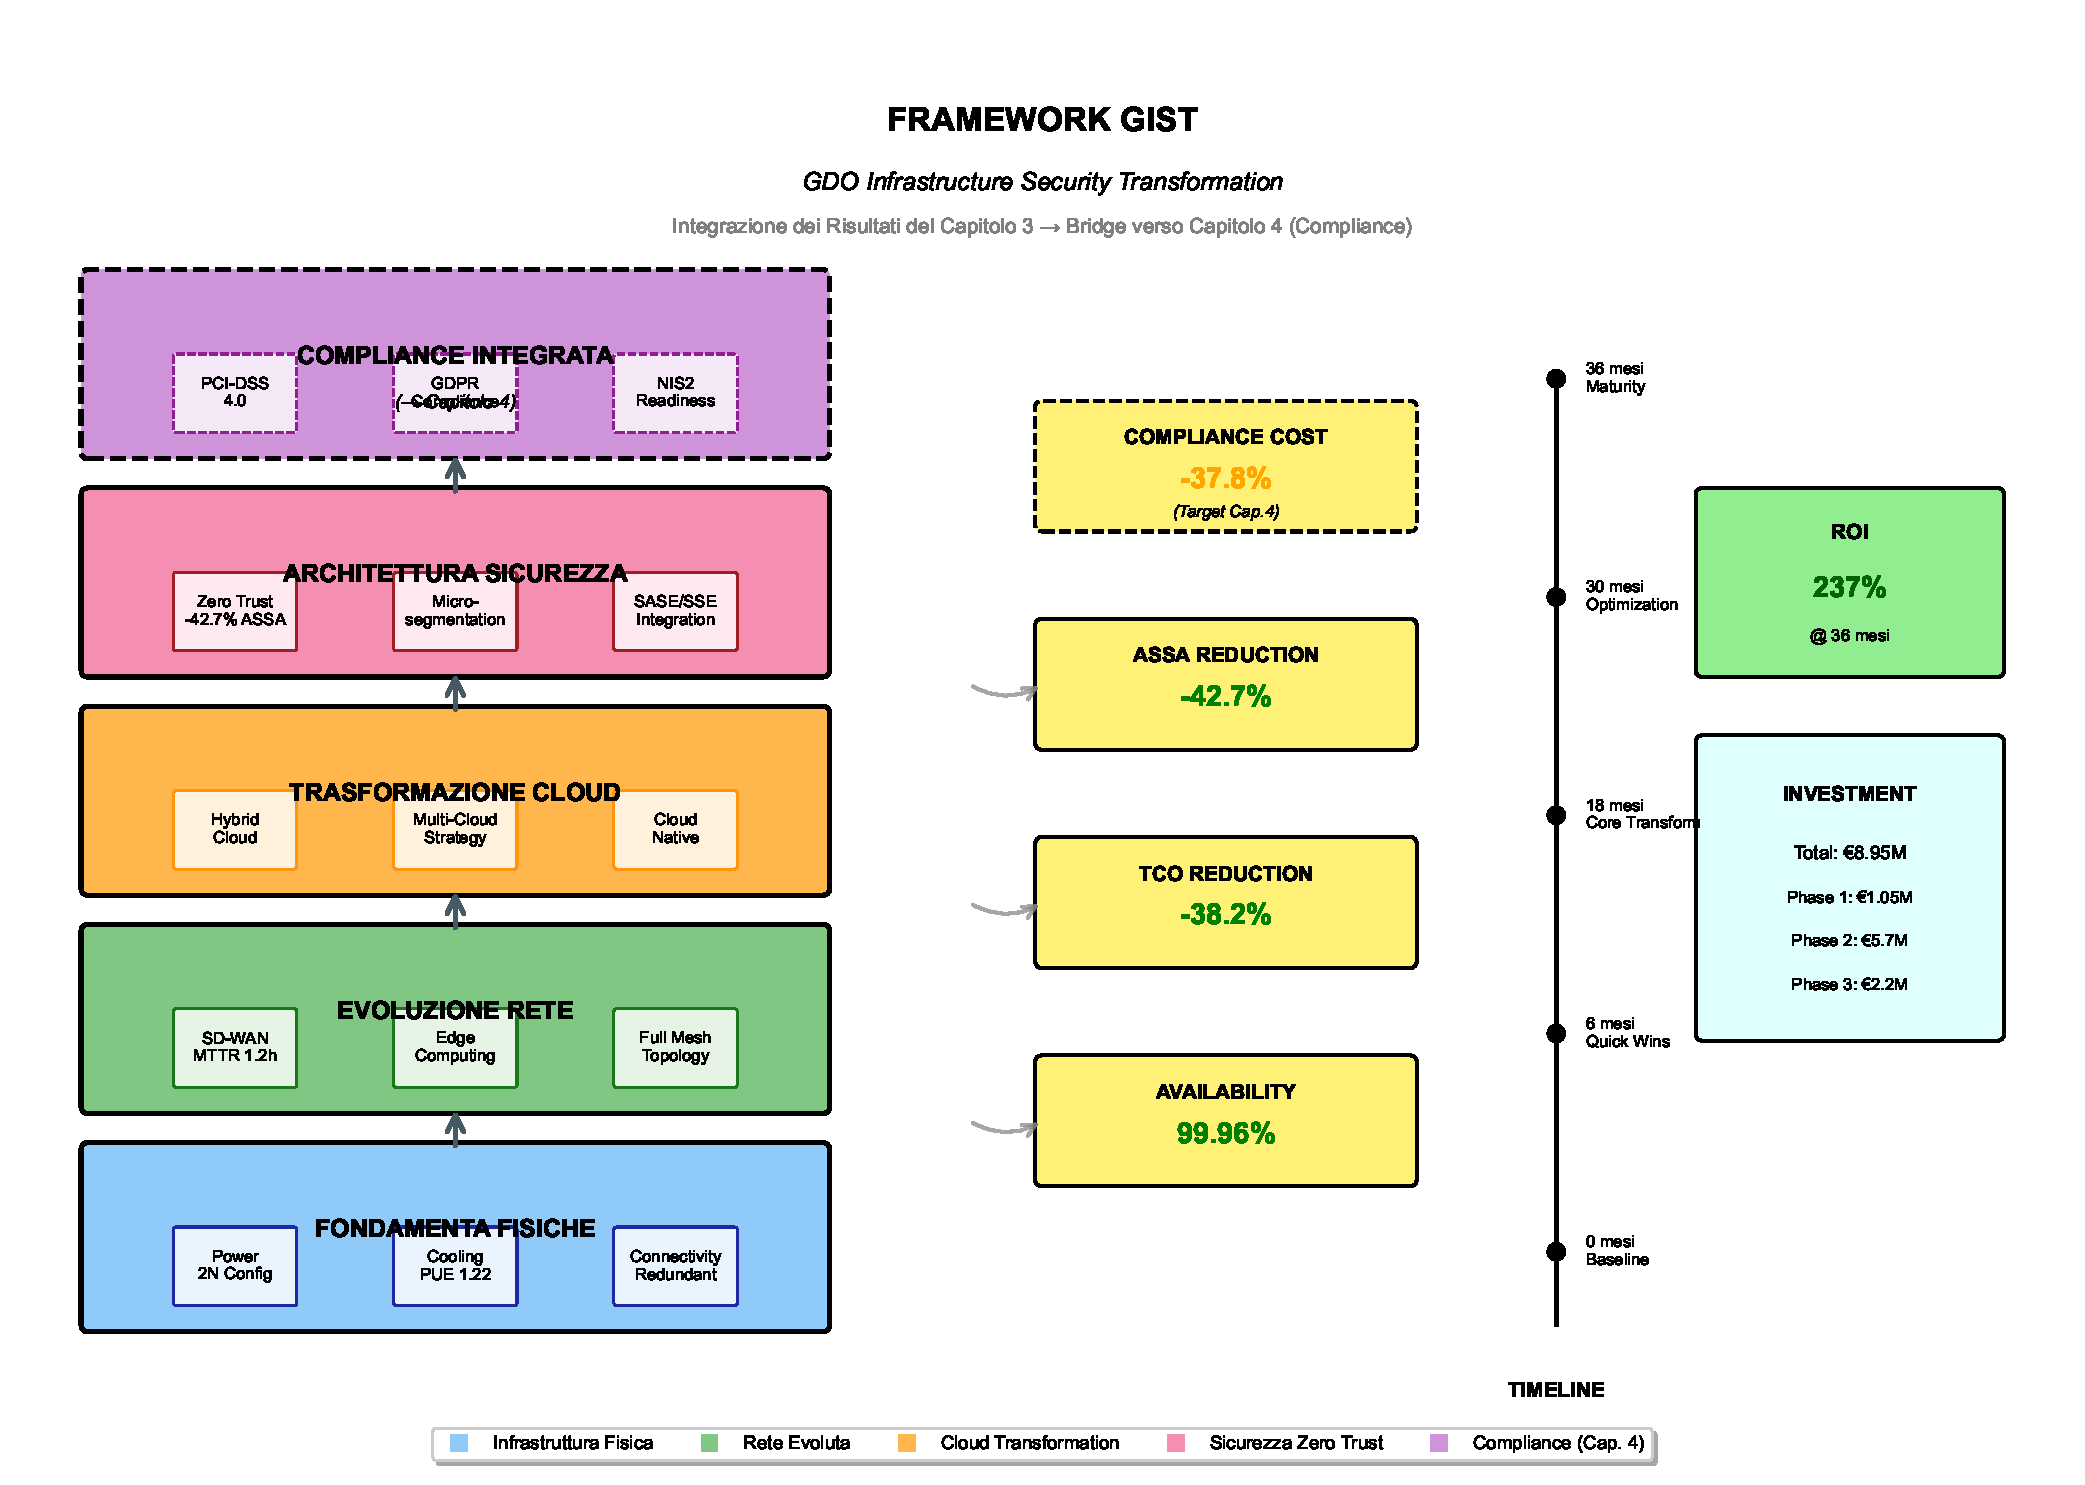
\includegraphics[width=\textwidth]{thesis_figures/cap3/figura_3_6_framework_integrato.pdf}
\caption{Framework GIST (\gls{gdo} Infrastructure Security Transformation): Integrazione dei risultati del Capitolo 3 e collegamento con le tematiche di Compliance del Capitolo 4. I cinque livelli mostrano l'evoluzione dalle fondamenta fisiche alla compliance integrata, con le metriche chiave validate attraverso simulazione Monte Carlo (10.000 iterazioni).}
\label{fig:framework_gist}
\end{figure}

\clearpage
\printbibliography[
    heading=subbibliography,
    title={Riferimenti Bibliografici del Capitolo 3},
]

%\endrefsection

\clearpage